
\begin{tabular}{ll}
\multicolumn{2}{l}{\textit{Setup: framework, curricula, data}} \\
A.1  & \hyperref[sec:lit-review]{Comparison of \beetle{} and L2LMs} \\
A.2  & \hyperref[sec:train]{\beetle{} Training Framework} \\
A.3  & \hyperref[sec:beetle-curricula]{\beetle{} Curricula and Control Parameters} \\
A.4  & \hyperref[sec:beetle-data]{Beetle-Data} \\
\addlinespace
\multicolumn{2}{l}{\textit{G. Statistical validation of MECO claims}} \\
A.5  & \hyperref[sec:meco-results]{Detailed MECO Results} \\
A.6  & \hyperref[sec:significance-comprehensive]{Statistical Significance Testing} \\
\addlinespace
\multicolumn{2}{l}{\textit{H. Robustness, hierarchical reconciliation \& supplementary tables}} \\
A.7  & \hyperref[sec:hier-model]{Hierarchical Model of Structured Variation} \\
A.8  & \hyperref[sec:supp-tables]{MECO Supplementary Tables} \\
\addlinespace
\multicolumn{2}{l}{\textit{J. Interpretability diagnostics (exploratory)}} \\
A.9  & \hyperref[sec:beetle-analyze]{Pico-Analyze Comparative Interpretability} \\
A.10 & \hyperref[sec:appx-dynamics]{Learning Dynamics} \\
\addlinespace
\multicolumn{2}{l}{\textit{K. Downstream tasks}} \\
A.11 & \hyperref[sec:downstream]{Detailed Downstream Results} \\
A.12 & \hyperref[sec:supp-results]{Supplementary BLiSS \& Pedagogical Results} \\
\addlinespace
\multicolumn{2}{l}{\textit{L. Cross-lingual / priming}} \\
A.13 & \hyperref[sec:priming]{Cross-lingual Structural Priming (B-GPT Comparison)} \\
\end{tabular}
 
\noindent\rule{\linewidth}{0.4pt}
 
 
% ####################################################################
% ===== APPENDIX SETUP: framework, curricula, data =====
% ####################################################################
% =====================================================================
\section{Comparison of \beetle{} and L2LMs}\label{sec:lit-review}
 
\begin{figure}[t!]
    \centering
    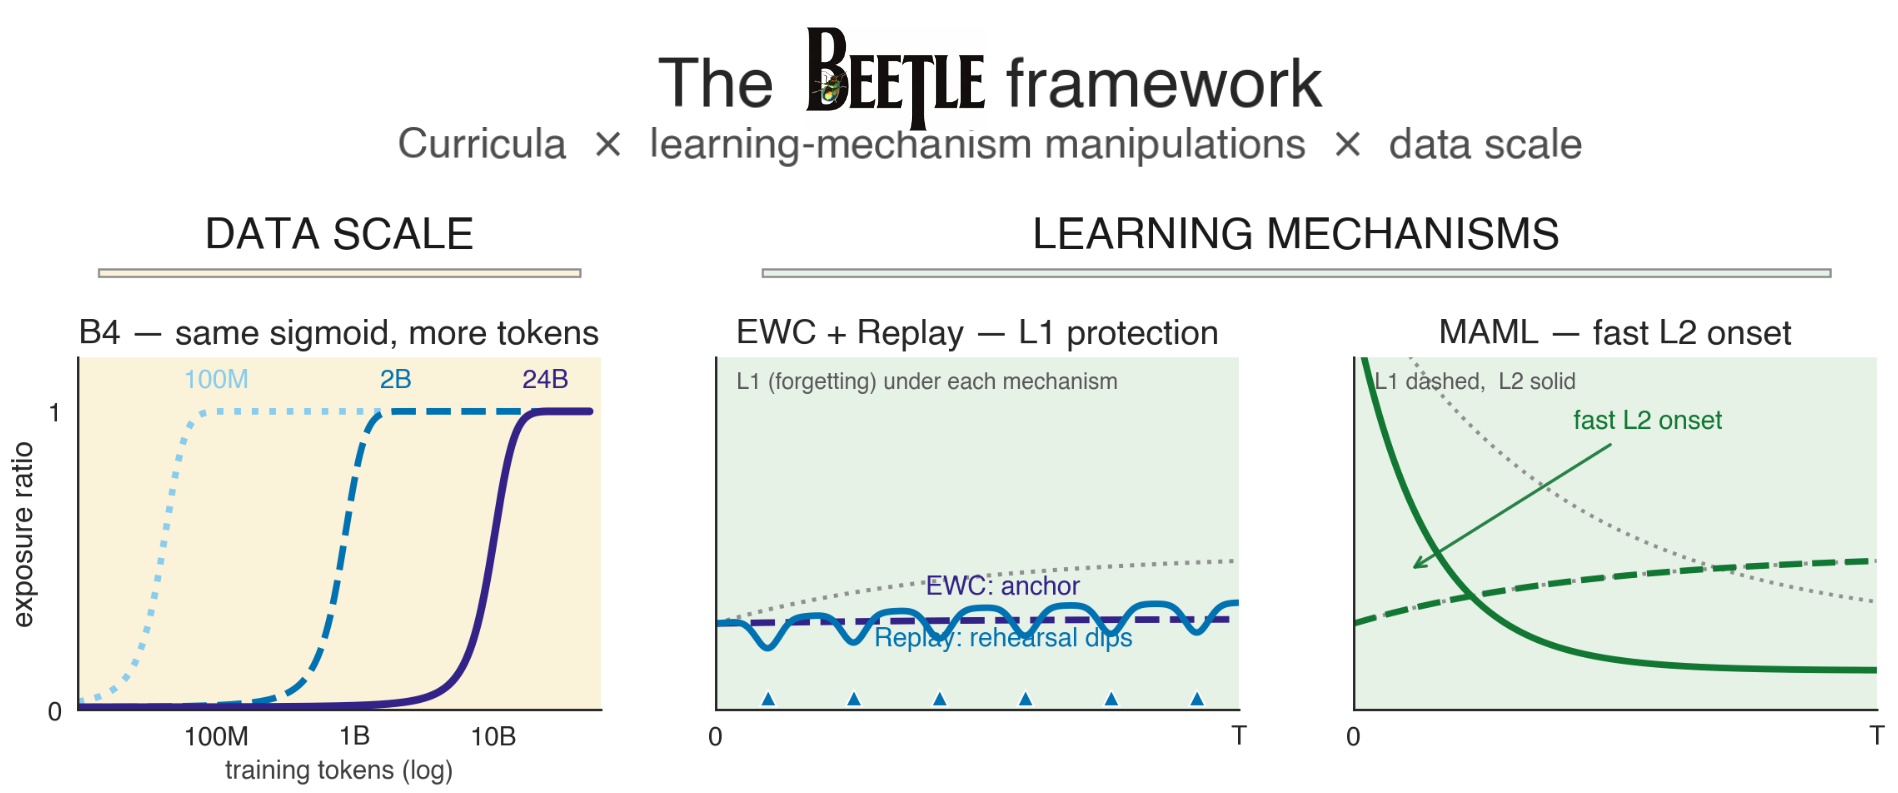
\includegraphics[width=0.85\linewidth]{fig/logo/3.png}
    \caption{Schematic comparison of the five \beetle{} bilingual exposure curricula B1--B5 (cf.\ Tab.~\ref{tab:taxonomy}). The L1:L2 token-mix trajectory across training is rendered for each curriculum: B2/B3 share a mid-training sigmoid L2-onset, B5 a late (80\%-of-training) onset, and B4 a constant-mean-with-bursts schedule from step~0.}
    \label{fig:beetle}
\end{figure}
 
\begin{table}[!ht]
        \centering
        \small
        \begin{tabular}{lccccc c}
        \toprule
        \textbf{Work} & \textbf{S} & \textbf{CL} & \textbf{M} & \textbf{C} & \textbf{CF} & \textbf{Dim} \\
        \midrule
        Constantinescu et al.\ (2025) & W & -- & -- & EWC & -- & $\triangle$ \\
        Arnett et al.\ (2025)         & W & -- & \checkmark & -- & -- & $\triangle\triangle$ \\
        Aoyama et al.\ (2024)         & W & -- & -- & -- & RT & $\triangle$ \\
        Diehl Martinez et al.\ (2025) & W & -- & -- & -- & -- & $\triangle\triangle$ \\
        Anon.\ (2025)                 & H & \checkmark & \checkmark & -- & -- & $\triangle\triangle\triangle$ \\
        Diehl Martinez et al.\ (2023) & H & \checkmark & -- & -- & -- & $\triangle\triangle\triangle$ \\
        Mita et al.\ (2025)           & H & -- & -- & -- & WM & $\triangle\triangle$ \\
        \midrule
        \textbf{BeetleLM}
        & \textbf{H+W}
        & \checkmark
        & \checkmark
        & \checkmark
        & \checkmark
        & $\triangle\times7$ \\
        \bottomrule
        \end{tabular}
        \caption{\beetle{} against prior bilingual / L2 language-model work. \textbf{S}: scale regime (W = web-scale, H = human-scale, H+W = both). \textbf{CL}: continual-learning controls. \textbf{M}: meta-learning. \textbf{C}: explicit catastrophic-forgetting controls. \textbf{CF}: catastrophic-forgetting evaluation. \textbf{Dim}: number of evaluation dimensions.}
        \label{tab:curricula-overview}
\end{table}
 
Bilingual and second-language language models (L2LMs) have been explored through a range of architectural and training regimes aimed at simulating second language acquisition, while increasingly serving as testbeds for cognitively grounded evaluation via surprisal-based reading-time prediction. Early computational approaches framed second-language acquisition as sequential adaptation in probabilistic or neural models \citep{matusevych-etal-2013-computational}, while more recent work formalises bilingual training as controlled pretraining or adaptation in large language models. \citet{aoyama2024modeling} propose a two-phase regime in which a model is first trained on L1 data and then adapted to L2 while freezing most parameters except embeddings and the LM head, showing that constrained plasticity can preserve prior knowledge while enabling new-language acquisition. \citet{constantinescu2025investigating} extend this direction by systematically varying exposure schedules and loss functions, including Elastic Weight Consolidation, to study stability–plasticity trade-offs under continual bilingual training. \citet{arnett-etal-2025-acquisition} introduce B-GPT and contrast sequential versus simultaneous bilingual pretraining, finding that mixed exposure better approximates naturalistic bilingual learning dynamics, while \citet{feng2026bilingual} study scaling in bilingual machine-translation settings and show that data composition and scale strongly influence cross-lingual transfer, albeit under primarily task-based evaluation. Earlier multilingual child-directed-speech L2LMs \citep{yadavalli-etal-2023-slabert, oba-etal-2023-second} explore similar ideas but remain limited in language coverage, checkpointing, and evaluation depth.
 
A key motivation for these models is their use as cognitive proxies through surprisal-based reading-time prediction, where processing difficulty is linked to a word’s unexpectedness under a language model, formalised as $-\log P(w_i \mid w_{<i})$. This framework underlies psycholinguistic models of reading time and is typically operationalised via regression models that combine surprisal with lexical covariates, evaluated through the change in log-likelihood ($\Delta\log L$) between baseline and surprisal-augmented models \citep{wilcox2020predictive, kaye2025sentence}. Psychometric predictive power is not a simple function of model quality; instead, it reflects how well model probabilities align with human processing distributions \citep{de-varda-marelli-2022-effects, goodkind2018predictive, shain2024large}. Despite extensive work in L1 psycholinguistics, comparatively little work has examined L2 cognitive modelling with language models, even though L2 reading exhibits systematic cross-linguistic variation and proficiency effects \citep{hillert1998sentence, meister2021revisiting, kuribayashi-etal-2021-lower}.
 
Against this backdrop, \beetle{} extends prior L2LM work in three ways. First, it specifies eight typologically diverse L1s for this paper (three released bilingually at FineWeb scale, five corpus-prepared; the framework pool spans 38 languages), parameterises exposure along six continuous dimensions rather than binary sequential/simultaneous splits, and integrates cognitively and pedagogically grounded evaluations including MECO L2 reading times, BLiSS, and CEFR proficiency measures. Second, its continual-learning framework unifies prior isolated strategies: Elastic Weight Consolidation, MAML-style adaptation, and learning-rate plasticity subsume earlier single-method approaches such as \citet{constantinescu2025investigating}, while embedding-and-LM-head-only adaptation \citep{aoyama2024modeling} appears as a special case within \beetle{}’s fifteen training regimes. Third, unlike prior work focused on limited bilingual corpora or synthetic machine-translation settings, \beetle{} evaluates models trained on large-scale real web data (FineWeb) across 100M, 2B, and 24B token regimes, directly linking scaling, cross-lingual transfer, and reading-time predictive power within a unified evaluation framework.
 
\paragraph{Surprisal theory.} Following Surprisal Theory \citep{hale2001probabilistic, levy2008expectation}, processing effort at word $w_i$ is the negative log-probability of the word given preceding context,
\[
\mathrm{surprisal}(w_i) = -\log_2 P(w_i \mid w_1, w_2, \dots, w_{i-1}),
\]
which links measured cognitive effort to predictability. Following \citet{wilcox2020predictive} and \citet{kaye2025sentence}, we measure predictive power for observation $i$ as the change in log-likelihood between a target regression (controls plus surprisal) and a baseline regression (controls only):
\begin{equation}
\Delta\mathrm{LL}_i =
\log L_{\text{target}}(RT_i \mid x_{\text{target}})
- \log L_{\text{baseline}}(RT_i \mid x_{\text{baseline}}),
\end{equation}
where $RT_i$ is a single participant's reading time on a word, $x_{\text{baseline}}$ are the control predictors, and $x_{\text{target}}$ adds surprisal. Exact \texttt{R} formulae are given in App.~\ref{sec:meco-results}.
 
\paragraph{Learning dynamics, cognates, BLiSS.} \citet{aoyama-wilcox-2025-language} place the monolingual predictive-power tipping point at ${\sim}2$B tokens; we test whether structured-exposure curricula delay or eliminate this decay under bilingual training. \citet{aoyama2025predicting} show induction-head emergence is data-property-driven; we quantify how exposure curriculum shifts emergence timing across L1 and L2. \citet{frank2026dutch} report Dutch--English cognate / false-friend effects, which we connect to MECO~L2 reading. The BLiSS task and dataset are due to \citet{gao2025bliss}: a CEFR-stratified discrimination of artificial versus learner errors. We adopt their NGS / CPS / RP$@\tau$ protocol unchanged and sweep it across our curriculum grid.
 
\paragraph{Pedagogical CEFR simulation and cognitive constraints.} \citet{benedetto-etal-2024-using} score frontier LMs on the CUP\&A5 dataset \citep{mullooly2023cupa5} using $M = \rho_{L,I} - P$, with $\rho_{L,I}$ the Spearman correlation between simulated CEFR-level accuracy and item difficulty and $P$ a non-monotonicity penalty; they simulate CEFR via prompting, whereas \beetle{} simulates it via training-time exposure curricula. Cognitive-constraint priors --- Shuffle-Dyck pre-pretraining \citep{hu2025between} and ALiBi-decay working memory \citep{mita2025wm, madhayastha2026wm} --- are implemented as opt-in modules in the architecture registry rather than as principal contributions.
 
 
% =====================================================================
\section{\beetle{} Training Framework}\label{sec:train}
 
\beetle{} is built on a custom \textsc{Pico} decoder stack \citep{diehl-martinez-etal-2025-pico} with curriculum-aware checkpointing, a registry of fifteen continual-learning strategies, and a tokeniser layer supporting per-language, shared-bilingual, and shared-trilingual vocabularies. The composable schedule primitives that govern multilingual exposure (\textsc{ConstantExposure}, \textsc{SigmoidRamp}, \textsc{LinearRamp}, \textsc{BurstSchedule}, \textsc{CyclicalSchedule}, \textsc{CompositeSchedule}) and the optional \textsc{EpisodicSampler} that groups consecutive batches into named contexts (\emph{home} vs.\ \emph{classroom}) implement the full enumeration described in the body. Ten predefined acquisition conditions map psycholinguistic scenarios to concrete schedule parameters.
 
\subsection{Architecture Registry}\label{sec:beetle-architecture-registry}
 
The body backbone is \texttt{PicoDecoder}, a LLaMA-style \citep{touvron2023llama} decoder with $L=14$ blocks, RMSNorm \citep{zhang2019rms}, grouped-query attention \citep{ainslie2023gqa} (12 query heads, 1 key/value head), rotary position embeddings \citep{su2024rope}, and SwiGLU feed-forward \citep{shazeer2020glu} expanding to $4d$ and projecting back to $d$. The shared bilingual vocabulary used in the main runs has size $50{,}304$; per-language and shared-trilingual tokenisers are configured separately. Sequence length is $512$ under BF16-mixed precision. Width is the only scale-dependent hyper-parameter: $d\in\{96,384,768,1536\}$ for the tiny, small, medium, and large variants. The 125M-parameter ``medium'' variant ($d=768$, 12 heads, 1 KV head, 14 layers) is used for every reported run. Complementary architectures enable controlled comparisons across inductive biases: \textbf{BGPT}, a GPT-2-style decoder with learned positional embeddings used in \citet{arnett-etal-2025-acquisition}; \textbf{BeetleMoE}, a top-$k$ mixture-of-experts model with ST-MoE auxiliary routing losses; and \textbf{BeetleSSM}, which replaces attention blocks with Mamba-style state-space modules. Pre-pretraining (Shuffle-Dyck) and time-varying ALiBi slopes are implemented as opt-in overlays inside the registry and are not used in the main runs.
 
\subsection{Continual-Learning Strategies}\label{sec:cl-strategies}
 
\beetle{} bundles \textbf{fifteen} modular continual-learning strategies in five families. \emph{Parameter regularisation}: EWC \citep{kirkpatrick2017overcoming} with $\lambda\in[0,40]$ and a Fisher snapshot at phase change, SI (synaptic intelligence), and MAS (memory-aware synapses). \emph{Generative and similarity replay}: LAMOL \citep{sun2020lamol} with $\lambda_{\text{replay}}\in[0,0.5]$, InsCL-style similarity replay (cosine and Wasserstein centroids), and episodic-sample replay buffers. \emph{Meta-learning}: first-order MAML / SMLMT \citep{bansal-etal-2020-self,africa-etal-2025-learning,africa-etal-2025-meta} with hybrid ratio $\in[0,0.4]$ and $N$-way/$k$-shot inner episodes. \emph{Distillation}: feature-level (FitNets), output-level (Hinton-KD), and self-distillation against the pre-L2 anchor. \emph{Architectural and auxiliary-loss}: TILT freeze-and-extend, exposure-LR plasticity boost (\texttt{plasticity\_boost}$\in[1,3]$), ALiBi-scheduler decay, and Shuffle-Dyck pre-pretraining. The B1--B5 grid reported in the body uses three of these (EWC, LAMOL, LR-plasticity); the remaining twelve are reproducible from the released configuration files. Tab.~\ref{tab:cl-registry} summarises the registry.
 
\begin{table*}[t]
\centering
\small
\setlength{\tabcolsep}{3.5pt}
\begin{tabular}{llll}
\toprule
\textbf{Family} & \textbf{Strategy} & \textbf{Mechanism} & \textbf{Key hyperparameters} \\
\midrule
\multicolumn{4}{l}{\textit{Parameter regularisation}} \\
& EWC \citep{kirkpatrick2017overcoming} & Diagonal-Fisher quadratic penalty at phase change & $\lambda\in[0,40]$, $K_{\text{Fisher}}=10$ \\
& SI & Online importance accumulation & $c$, damping \\
& MAS & Gradient-magnitude importance & $\lambda$ \\
\midrule
\multicolumn{4}{l}{\textit{Replay}} \\
& LAMOL \citep{sun2020lamol} & Pseudo-sample generation, nucleus sampling & $\lambda_{\text{replay}}\in[0,0.5]$, top-$p$ \\
& InsCL similarity replay & Centroid-similarity weighted replay & cosine/Wasserstein, buffer size \\
& Episodic replay & Stored exemplars, uniform sampling & buffer size, mix ratio \\
\midrule
\multicolumn{4}{l}{\textit{Meta-learning}} \\
& MAML / SMLMT & Inner-loop adaptation on (S,Q) splits & hybrid ratio $\in[0,0.4]$, $N$-way, $k$-shot \\
\midrule
\multicolumn{4}{l}{\textit{Distillation}} \\
& Hinton-KD & Soft-target cross-entropy against pre-L2 anchor & $T$, $\lambda_{KD}$ \\
& Self-distillation & Same model as teacher at earlier checkpoint & ckpt offset \\
& FitNets feature distill. & Hidden-state $\ell_2$ alignment & layer-pair list \\
\midrule
\multicolumn{4}{l}{\textit{Architectural / auxiliary-loss}} \\
& TILT freeze-and-extend & Freeze backbone; train embed + LM head & frozen modules \\
& Exposure-LR plasticity & Token-exposure LR with phase-transition boost & boost $\in[1,3]$, warmup tokens \\
& ALiBi scheduler & Time-varying ALiBi slopes across phases & initial/final slope, decay shape \\
& Shuffle-Dyck pre-pretraining & Formal-language warmup before NL & steps, depth \\
& EWC + MAML stack & Composite of regularisation + meta-learning & paired hyperparameters \\
\bottomrule
\end{tabular}
\caption{The fifteen continual-learning strategies in the \beetle{} registry. The reported B1--B5 grid uses EWC, LAMOL, and exposure-LR plasticity overlays; the remaining twelve are reproducible from the released configuration files.}
\label{tab:cl-registry}
\end{table*}
 
 
% =====================================================================
\section{\beetle{} Curricula and Control Parameters}\label{sec:beetle-curricula}
 
%\paragraph{Bilingual conditions (B1--B5).} The five bilingual exposure schedules used in every reported run differ along three axes: \emph{L2 onset timing} (immediate / mid-training / late), \emph{final L1:L2 ratio} (50:50 / 80:20), and \emph{transition sharpness} (sharp vs.\ sigmoid). \textbf{B1 Balanced}: 50:50 L1:L2 throughout (from step 0). \textbf{B2 Simultaneous}: 100\% L1 until 50\% of training, then a sigmoid ramp to 50:50. \textbf{B3 Sequential}: 100\% L1 until 50\% of training, then $\{0{:}100, 33{:}67, 50{:}50\}$ L1:L2 in three onset-ratio variants (B3-0 / B3-33 / B3-50). \textbf{B4 Classroom}: episodic L2 bursts, 80:20 token budget. \textbf{B5 Late}: L2 introduced at 80\% of training. All conditions hold the total token budget constant at the per-pair scale (100M HumanScale, 2B FineWeb-2B, 24B FineWeb-24B) and share the \texttt{PicoDecoder} backbone of App.~\ref{sec:beetle-architecture-registry}.
 
The B4 classroom runs set \texttt{ewc.enabled: false}, as does the B2 base condition, so the B2-vs-B4 timing-versus-proportion contrast carries no EWC asymmetry on either side.
 
\paragraph{Trilingual conditions (T1--T4).}  \beetle{} additionally implements Trilingual Curricula, which are not explored in this paer due to limited reading time and psycholinguistic data. \textbf{T1 Simultaneous Trilingual}: ${\approx}33/33/33$ mixture, context-clustered batches. \textbf{T2 Sequential Trilingual}: $L_1\to L_2\to L_3$ via chained sigmoids. \textbf{T3 Heritage~$+\,L_3$}: $L_1\to L_2$ dominance $\to L_3$, with $L_1$ re-exposure. \textbf{T4 Dominant $L_2$ + Late $L_3$}: $L_2$ dominant, $L_1$ weak, $L_3$ introduced late. The trilingual configurations cover 18 orderings drawn from $\{\text{deu, eng, nld, zho}\}$.
 
\paragraph{Formalisation.} A bilingual curriculum is a time-dependent mixture $\mathcal{D}_{\text{mix}}(t) = \alpha(t)\,\mathcal{D}_1 \cup (1-\alpha(t))\,\mathcal{D}_2$, where $\alpha(t)\in[0,1]$ is the per-step L2 sampling probability and $t\in[0,T]$ indexes training. The polyglot generalisation is a language-exposure vector $\boldsymbol{\alpha}(t)=(\alpha_1(t),\ldots,\alpha_N(t))$ with $\sum_i \alpha_i(t)=1$. Each schedule maps a normalised progress value $p\in[0,1]$ to a per-language sampling weight; phase boundaries are discrete events that trigger EWC snapshots in continual-learning runs. Rather than specifying $\boldsymbol{\alpha}(t)$ as an arbitrary continuous function, we represent curricula as a sequence of discrete phases $\mathcal{C} = \{(\tau_k^{\text{start}}, \tau_k^{\text{end}}, \mathbf{w}_k)\}_{k=1}^{K}$, where $\mathbf{w}_k \in \mathbb{R}^N$ satisfies $\sum_i w_{k,i}=1$; for $\tau_k^{\text{start}} \le t/T < \tau_k^{\text{end}}$ we set $\boldsymbol{\alpha}(t) = \mathbf{w}_k$. This declarative phase representation is used in every reported run.
 
\begin{table}[t]
\centering
\small
\begin{tabular}{lccccc}
\toprule
\textbf{Factor} & \textbf{B1} & \textbf{B2} & \textbf{B3} & \textbf{B4} & \textbf{B5} \\
\midrule
L2 onset & step 0 & mid (50\%) & mid (50\%) & step 0 & late (80\%) \\
Final L2 ratio & 50\% & 50\% & 67\% & 20\% (mean) & 50\% \\
Transition & none & sigmoid & sigmoid & const.\ mean + bursts & sigmoid \\
Burst exposure & no & no & no & yes & no \\
Episodic clustering & no & no & no & yes & no \\
CL overlay & none & none & none & none & LR-boost \\
\bottomrule
\end{tabular}
\caption{Controlled curriculum factors across the five bilingual conditions B1--B5. Each condition varies a subset of factors while holding the remainder fixed. B4 sets \texttt{ewc.enabled: false} (as does the B2 base), so the B2-vs-B4 contrast carries no EWC asymmetry.}
\label{tab:taxonomy}
\end{table}
 
\paragraph{Ablation grid.} Tab.~\ref{tab:ablation-sweep} enumerates the eight nld--eng \textsc{HumanScale} variants that constitute the minimal ablation. Each variant is trained under three a-priori-fixed seeds $\{13, 42, 97\}$ to support a paired permutation test plus Cohen's $d_z$ with Holm--Bonferroni correction on the MECO~L2 alignment metric. Each variant trains on $8\times$A100 80~GB for ${\sim}1$~h.
 
\begin{table}[t]
\centering
\small
\caption{Minimal B1/B2/B3 ablation sweep on the nld--eng \textsc{HumanScale} pair. Eight variants $\times$ three seeds support paired-permutation significance tests on MECO~L2 $\Delta\log L$. LAMOL variants use $\lambda_{\text{replay}}=0.2$.}
\label{tab:ablation-sweep}
\begin{tabular}{@{}l l l@{}}
\toprule
Family & Variant & Manipulation (vs.\ base condition) \\
\midrule
B1 & B1        & Base balanced (50:50 throughout) \\
B1 & B1b       & Balanced with delayed L2 onset \\
\midrule
B2 & B2        & Base simultaneous (sigmoid from 50\%) \\
B2 & B2$+$EWC   & EWC regulariser at phase change \\
B2 & B2$+$LAMOL & LAMOL generative replay ($\lambda=0.2$) \\
B2 & B2$+$LR    & LR-plasticity boost at L2 onset \\
\midrule
B3 & B3        & Base sequential (33:67 post-transition) \\
B3 & B3-full   & Sequential with full EWC $+$ MAML $+$ LR stack \\
\bottomrule
\end{tabular}
\end{table}
 
 
% =====================================================================
\section{Beetle-Data}\label{sec:beetle-data}
 
%\paragraph{Source corpora and target budget.} Beetle-Data is the data-preparation procedure that produces every training corpus in the reported runs. Two source families are mined: \textbf{BabyBabelLM} \citep{jumelet2025babybabellmmultilingualbenchmarkdevelopmentally} for the \textsc{HumanScale} 100M-token regime, and FineWeb-Edu (English) plus FineWeb-2 (non-English) \citep{penedo2025fineweb2} for the \textsc{FineWeb} 2B and 24B regimes. The procedure streams raw documents, applies a 13-gram benchmark-overlap decontaminator, and pretokenises to Arrow shards compatible with the \textsc{BeetleLM} trainer. It cuts to a 24~B-token target per bilingual pair (12~B L1 + 12~B EN) at pretokenisation; the human-scale target is 100~M tokens (50:50) and the 2~B regime is 1~B~+~1~B.
 
%\paragraph{Per-language token counts.} Table~\ref{tab:beetle-data-tokens} reports the per-language token budget at each regime. The HumanScale budget of 50~M tokens per side mirrors the BabyBabelLM Tier-1 cap; FineWeb-24B uses 12~B per side, sized to Chinchilla-optimal for the 125M-parameter backbone \citep{hoffmann2022}.

\paragraph{Deduplication, quality, tokeniser.} Within each language, decontaminated documents are deduplicated via SHA-256 hashing of the first 512 tokens. For the main runs we use the static (non-curriculum) procedure; a curriculum-graded variant is reserved for future work. Each bilingual pair uses a $50{,}000$-vocab BPE tokeniser trained jointly on a $1{:}1$ L1:English mixture and shared across both orderings; monolingual anchors use a $32{,}000$-vocab tokeniser; trilingual experiments reuse a single $32{,}768$-vocab trilingual tokeniser to remove vocabulary as a confound in catastrophic-forgetting analyses. Decontaminated Parquet shards (28~B tokens per language side) and pretokenised Arrow datasets (cut to 24~B per pair) are released publicly, together with per-run manifests recording the document-to-shard mapping and the contamination rate for each run.
 
 
% ####################################################################
% ===== BLOCK G --- STATISTICAL VALIDATION OF MECO CLAIMS =====
% ####################################################################
% =====================================================================
\section{Detailed MECO Results}\label{sec:meco-results}
 
This appendix evaluates how bilingual training curricula affect alignment between language-model surprisal and human L2 reading times in MECO. Two results hold. Staged bilingual exposure (B2/B3/B5) improves first-pass reading-time alignment relative to balanced exposure, decisively for Germanic L1 readers and across training scales. Separately, under matched (sum-of-subwords) aggregation, 125M matched bilinguals are competitive with much larger multilingual LLMs on MECO alignment; this is a confounded cross-class comparison whose magnitude is aggregation-dependent (the sensitivity analysis below), so we read it as a reference point and draw no scale or cross-class ranking from it. Every primary curriculum claim is within-\beetle{}, on the matched diagonal, under one shared tokeniser and aggregation.
 
\subsection{Metric and mixed-effects specification}\label{sec:meco-metric-app}
 
We quantify LM--human alignment as the improvement in mixed-effects fit from adding surprisal predictors to a baseline reading-time regression:
\[
\Delta\log L = \log L(\text{full}) - \log L(\text{baseline}).
\]
Larger values indicate that model surprisal explains additional variance in MECO reading times beyond standard lexical covariates. Both models are \texttt{lme4} fits on the wave-1$+$wave-2 joined first-pass data (\texttt{firstrun.dur}); the surprisal block is the only difference. Exact formulae:
\begin{equation}
\label{eq:full-model}
\begin{split}
\mathrm{firstrun\_dur} \sim{}&
\mathrm{scale}(\mathrm{Surprisal})
+ \mathrm{scale}(\mathrm{Surp1p})
+ \mathrm{scale}(\mathrm{Surp2p}) \\
&+ \mathcal{C}
+ (1 + \mathcal{C} \mid \mathrm{subid})
\end{split}
\end{equation}
\begin{equation}
\label{eq:meco-spec}
\mathrm{firstrun\_dur} \sim
\mathcal{C}
+ (1 + \mathcal{C} \mid \mathrm{subid})
\end{equation}
where $\mathcal{C}$ is the shared lexical-covariate block (word position; word length and frequency, each with two prior-word lags), \texttt{Surp1p}/\texttt{Surp2p} are surprisal lags, and \texttt{subid} is the participant. Fits use restricted-maximum-likelihood estimation disabled (\texttt{REML=FALSE}) with uncorrelated by-subject random slopes; the fitting script is released with the code. Per-cell sample sizes are on the order of tens of subjects and tens of thousands of word-level observations (the matched-Dutch condition has $46$ subjects, $n_{\text{obs}}{\approx}29{,}900$). Per-language rankings (Tab.~\ref{tab:meco}) average $\Delta\log L$ over reader-L1s within each (model, L2-language) cell; the participant-pooled Spearman cross-check (Tab.~\ref{tab:meco_english_l2_participants}) confirms the principal difference is not driven by a few unusual readers.
 
\subsection{Headline curriculum results}\label{sec:meco-headline-app}
 
The matched-L1 curriculum comparison (Tab.~\ref{tab:meco_curriculum_matched}, main text, across the 100M/2B/24B scales) is the central result: each \beetle{} bilingual is trained on L1$\to$English and evaluated against the reading times of the matching L2 reader population. Staged curricula (B2/B3/B5) yield the strongest alignment on the Dutch and German cells, with sequential (B3-33) and late-onset (B5) highest and balanced exposure (B1) weakest at human scale; this Germanic staged-over-balanced ordering is preserved at the 2B and 24B scales (Dutch throughout; German at every scale except the 2B B5 cell). Chinese is mixed: balanced (B1) is competitive at every scale, with no curriculum uniformly ahead. Because each curriculum is currently represented by a single seed, these results establish a robust curriculum-associated effect; the timing-isolation ablation below (\S\ref{sec:timing-isolation}) is designed to separate exposure timing from the trajectory-integrated token mixture a schedule induces. The same Germanic curriculum ordering appears across training scales (Fig.~\ref{fig:fig1_scaling_x_curriculum}, main body).
 
\subsection{Timing-isolation ablation}\label{sec:timing-isolation}
 
The matched curriculum comparison bundles \emph{when} L2 arrives with the trajectory-integrated token mixture a schedule induces, so on its own it cannot attribute the MECO effect to temporal arrangement rather than to the data distribution. We therefore run a follow-up that holds the token marginal fixed and varies \emph{only} the temporal arrangement of identical tokens.
 
\paragraph{Design.} Five arms (T0--T4; Tab.~\ref{tab:tiso_design}) are trained on the matched nld--eng HumanScale setup, each a copy of the B1 configuration with \emph{only} the exposure schedule changed: identical architecture, tokeniser, optimiser, token budget, and the \emph{same} pretokenised L1/L2 shards (one shared cache), so every arm consumes the same token multiset. Because the data sampler is a deficit ratio-tracker driving the cumulative L1:L2 share toward the schedule's \emph{late} instantaneous target (not its time-integral), each arm's realised marginal is verified by simulation before training and held at $0.50$ (Tab.~\ref{tab:tiso_design}, ``Realised L2''); any arm drifting more than $0.01$ from $0.50$ is rejected. With the marginal matched by construction, a between-arm difference in $\Delta\log L$ is attributable to exposure \emph{timing}, not to how much or which L2 was seen.
 
\begin{table}[!ht]
  \centering \small
  \caption{\textbf{Timing-isolation arms (nld--eng, HumanScale 100M).} All arms share architecture, tokeniser, optimiser, token budget, and the same pretokenised shards; only the exposure schedule $w_{\mathrm{L2}}(t)$ differs. ``Realised L2'' is the cumulative L1:L2 token share produced by the sampler (ratio-tracker simulation over $10^4$ steps), verified at $0.50$ before training.}
  \label{tab:tiso_design}
  \begin{tabular}{@{}llcl@{}}
    \toprule
    Arm & Exposure schedule $w_{\mathrm{L2}}(t)$ & Real.\ L2 & Isolates \\
    \midrule
    T0 \textsc{iid}      & constant $0.5$                       & $0.500$ & reference (none) \\
    T1 \textsc{smooth}   & L1-only $\rightarrow$ 50:50 (sigmoid) & $0.497$ & gradual onset \\
    T2 \textsc{burst}    & square wave $0 \leftrightarrow 1$     & $0.500$ & burstiness \\
    T3 \textsc{block}    & L1-only -- L2-only halves             & $0.500$ & maximal staging \\
    T4 \textsc{shuffled} & T3 per-step stream permuted           & $0.499$ & order (vs.\ T3) \\
    \bottomrule
  \end{tabular}
\end{table}
 
\paragraph{Contrasts and pre-registered decision rule.} The arms license four contrasts: \textbf{T0 vs.\ \{T1,T2,T3\}} (does any temporal structure beat IID at a fixed marginal?); \textbf{T3 vs.\ T4} (same per-step mixtures, only the order differs --- isolates temporal \emph{order}); \textbf{T2 vs.\ T1} (burstiness vs.\ smooth onset); and \textbf{T2 vs.\ T0}. We pre-register both outcomes: if T2$\,{\approx}\,$T3$\,{>}\,$T0 and T3$\,{>}\,$T4, exposure timing contributes independently of the marginal; if T0$\,{\approx}\,$T1$\,{\approx}\,$T2$\,{\approx}\,$T3$\,{\approx}\,$T4, the principal curriculum effect reflects the induced mixture rather than timing, which we will report as such. FLORES perplexity is reported per arm to re-test the quality--alignment dissociation at a matched marginal.
 
% Results to be added on completion of the timing-isolation runs.
\begin{table}[!ht]
  \centering \small
  \caption{\textbf{Timing-isolation results (nld--eng HumanScale, seed 42).} MECO~$\Delta\log L$ (canonical procedure), BLiSS RP$@0$, and FLORES per-token surprisal per arm, with paired-bootstrap $95\%$ CIs on the key contrasts.}
  \label{tab:tiso_results}
  \begin{tabular}{@{}lccc@{}}
    \toprule
    Arm & MECO $\Delta\log L$ & BLiSS RP$@0$ & FLORES (nats/tok) \\
    \midrule
    T0 \textsc{iid}      & --- & --- & --- \\
    T1 \textsc{smooth}   & --- & --- & --- \\
    T2 \textsc{burst}    & --- & --- & --- \\
    T3 \textsc{block}    & --- & --- & --- \\
    T4 \textsc{shuffled} & --- & --- & --- \\
    \midrule
    \multicolumn{4}{@{}l}{\textit{Key contrasts (paired bootstrap 95\% CIs):}} \\
    \multicolumn{4}{@{}l}{\quad T0\,vs\,T3 (staging)\ \textbar\ T3\,vs\,T4 (order)\ \textbar\ T2\,vs\,T1} \\
    \bottomrule
  \end{tabular}
\end{table}
 
\subsection{Comparison to multilingual baselines}\label{sec:meco-baselines-app}
 
Under the matched (sum-of-subwords) aggregation, 125M matched bilinguals are competitive with much larger multilingual LLMs on MECO alignment. This compares systems differing in tokeniser, architecture, objective, and data, and the magnitude of the gap is not robust to the aggregation choice. We therefore read the comparison as a reference point only; the primary curriculum claims are all within-\beetle{}.
 
\paragraph{Sensitivity to subword aggregation.} Cross-class comparisons mix tokenisers, so we ran a first-subword-only vs.\ sum-of-subwords sensitivity check on the matched-Dutch BLOOM-7b1 vs.\ B3-33 nld--eng HS cell through the same canonical $\Delta\log L$ procedure ($n_{\text{obs}}{\approx}29{,}900$, $46$ subjects). Re-running surprisals reproduces the reported values to within ${\sim}3\%$ (B3-33 $135.6$ vs.\ released $139.6$; BLOOM-7b1 $20.5$ vs.\ $19.7$). Under first-subword-only aggregation, B3-33 falls to $7.0$ (retaining $5\%$ of its sum-of-subwords $\Delta\log L$) and BLOOM-7b1 to $14.9$ (retaining $73\%$): the cross-class gap of $+115~\Delta\log L$ becomes $-8~\Delta\log L$, a sign flip. The $>$100-$\Delta\log L$ cross-class statement is therefore specific to sum-of-subwords aggregation. Every within-\beetle{} cell shares one tokeniser and aggregation and is unaffected.
 
Tab.~\ref{tab:meco_baseline_comparators} sets the matched-L1 \beetle{} winner for each reader against the legacy BLOOM ladder (up to 7.1B) and a cohort of modern multilingual LLMs (up to 9B). Under sum-of-subwords aggregation the 125M matched bilingual is competitive with the larger models on the Germanic readers and with the strongest legacy comparator on Chinese. Per the sensitivity analysis above, this ordering is aggregation-dependent.
 
\begin{table}[!ht]
  \centering
  \small
  \caption{\textbf{MECO~L2 $\Delta\log L$: \beetle{} matched bilinguals vs.\ baselines.} \beetle{} rows report the matched-L1 winner per reader (from Tab.~\ref{tab:meco_curriculum_matched}). Bold = best in column; this is a within-column ranking only and does not imply a matched comparison --- the LLM rows differ in architecture, tokeniser, and subword aggregation and are contextual, so a bolded 125M \beetle{} cell is not a controlled win over a larger LLM. The strongest cross-class comparator, Baichuan-7B, slightly exceeds \beetle{} on German.}
  \label{tab:meco_baseline_comparators}
  \begin{tabular}{lrrrr}
    \toprule
    Model & Params & Dutch & German & Chinese \\
    \midrule
    \multicolumn{5}{l}{\textit{Legacy multilingual (BLOOM ladder)}} \\
    BLOOM-560m            & 0.56B & 44 & 182 & 149 \\
    BLOOM-1b1             & 1.1B  & 41 & 180 & \textbf{164} \\
    BLOOM-1b7             & 1.7B  & 34 & 151 & 137 \\
    BLOOM-7b1             & 7.1B  & 20 & 116 & 85 \\
    \midrule
    \multicolumn{5}{l}{\textit{Modern multilingual LLMs}} \\
    XGLM-4.5B             & 4.5B  & 9  & 19  & 23 \\
    EuroLLM-9B            & 9.0B  & 12 & 93  & 51 \\
    Gemma-2-9B            & 9.0B  & 9  & 97  & 50 \\
    Qwen-3-8B             & 8.0B  & 12 & 109 & 56 \\
    Llama-3.1-8B          & 8.0B  & 11 & 97  & 55 \\
    Baichuan-7B           & 7.0B  & 88 & \textbf{185} & 31 \\
    \midrule
    \multicolumn{5}{l}{\textit{\beetle{} matched bilinguals (125M)}} \\
    B3-33 nld--eng        & 0.125B & \textbf{140} & ---          & --- \\
    B3-33 deu--eng        & 0.125B & ---          & 177          & --- \\
    B2 deu--eng FW        & 0.125B & ---          & 184.7        & --- \\
    B5 zho--eng           & 0.125B & ---          & ---          & 115 \\
    \bottomrule
  \end{tabular}
\end{table}
 
\subsection{Per-eye-measure $\Delta\log L$ breakdown}\label{sec:meco-stage-app}
 
\emph{Exploratory diagnostic (\S\ref{sec:sig-uncertainty}).} Relative to balanced exposure (B1), the simultaneous (B2), sequential (B3), and late-onset (B5) schedules increase $\Delta\log L$ on first-run duration and decrease it on refixations and regressions-in. B2 gains $+0.79$~SD on first-run duration (95\% CI $[+0.24, +1.33]$); B5 gains $+0.93$~SD ($[+0.43, +1.42]$). The matched late-measure interactions are uniformly negative (B2$\times$refixation $\beta^{z}={-}1.06$; B5$\times$regression $\beta^{z}={-}1.30$) and survive FDR correction.
 
The pattern is not a bilingual-pretraining artefact. We anchor against a same-architecture monolingual-English \beetle{} fit under the same curriculum~$\times$~measure interaction specification used in this subsection. \emph{This is a different specification from the canonical first-pass cell of Tab.~\ref{tab:meco_full_canonical}, where mono-eng HS Dutch $=65.13$}; under the interaction specification the mono-eng anchor reaches $\Delta\log L{\approx}138$ on Dutch first-run duration, B2 reaches monolingual performance (${\approx}136$), and B1 falls ${\approx}80$ units short. Adding an English-competence covariate weakens the B2 late-measure effect but leaves the B5 pattern strong (first-run $\beta^{z}={+}0.78$, $p{<}.001$; $\times$regression $-1.01$, $p{<}.001$). The pattern reproduces in HumanScale~100M (B2 first-run $\beta^{z}={+}2.09$) and FineWeb~100M ($\beta^{z}={+}0.91$), so it is not specific to curated text. The \textbf{B4 classroom condition} reproduces the pattern at smaller magnitude (first-run $+0.40$~SD, refixation $-0.77$), consistent with sensitivity to the timing of L2 concentration rather than the final exposure ratio. Fig.~\ref{fig:fig3_spillover_decay} shows this pattern: staged curricula concentrate the surprisal coefficient at lag~0, whereas balanced B1 produces a flatter, lag-distributed profile.
 
\begin{figure}[!ht]
    \centering
    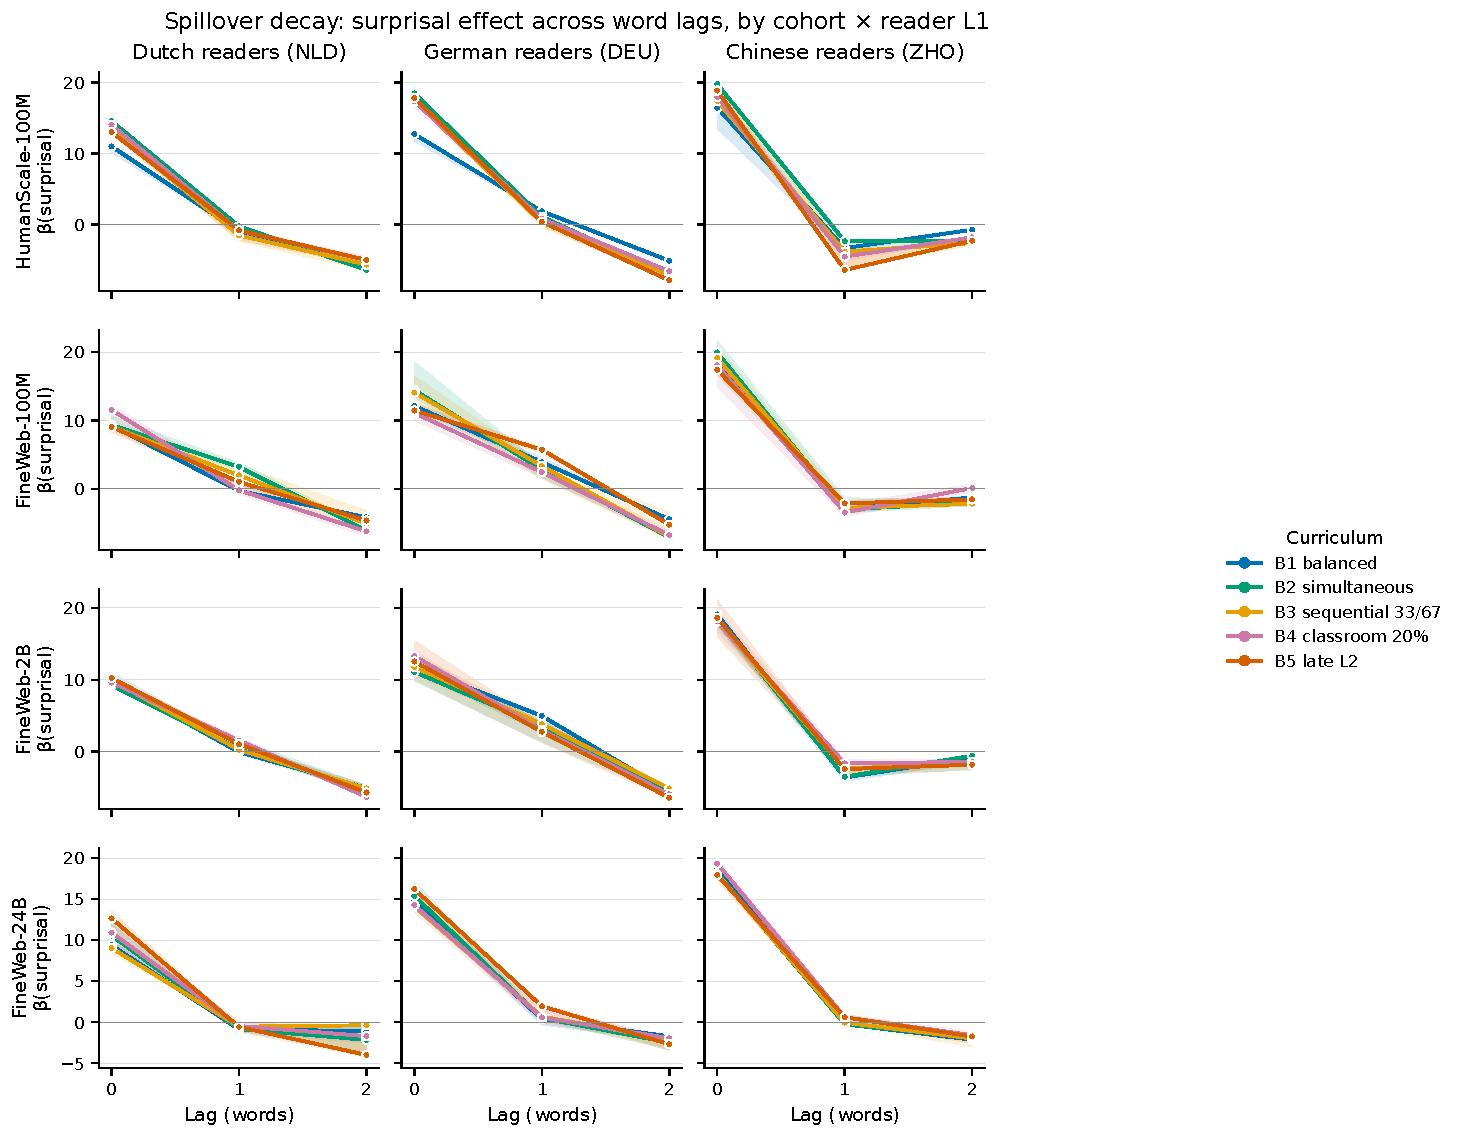
\includegraphics[width=\linewidth]{fig/meco/fig3_spillover_decay.pdf}
    \caption{\textbf{Spillover decay: $\beta$(surprisal) across word lags.} Per (training-token cohort, reader-L1) cell, $\beta$(surprisal) at lags 0--3 on first-run duration. Staged curricula (B2/B3-33/B5) concentrate the effect at lag~0; balanced B1 produces a flatter, lag-distributed profile. Lag-0 dominance grows with training tokens for Germanic L1s.}
    \label{fig:fig3_spillover_decay}
\end{figure}
 
\subsection{Likelihood decomposition and SAE ablation}\label{sec:meco-mech-app}
 
\emph{Two tiers (\S\ref{sec:sig-uncertainty}).} The context-share split below is a \emph{secondary} model-level result over the matched-\beetle{} set; the SAE ablation that follows is an exploratory single-model diagnostic. We treat the decomposition as descriptive statistics of each model's predictive distribution --- whether balanced and staged curricula draw their reading-time predictive gain from different horizons --- without positing a processing mechanism.
 
Using the context-share decomposition of App.~\ref{sec:beetle-analyze}, the dissociation is \emph{frequency vs.\ long-context, with the local component shared}. At the model level (one value per model averaged over the three MECO languages, a label-permutation test over models, continual-learning ablations excluded; Tab.~\ref{tab:sig_decomp_curriculum}), balanced curricula carry far more long-context share than staged --- $0.43$ vs.\ $0.09$ at FineWeb-100M ($\Delta{=}{+}0.34$, $p_\text{perm}{<}10^{-4}$), holding pooled across scales ($\Delta{=}{+}0.24$, $p_\text{perm}{<}10^{-4}$) and directionally consistent at 2B and 24B --- with the mirror-image split on the frequency component ($0.10$ vs.\ $0.47$ at 100M, $p_\text{perm}{=}6{\times}10^{-5}$). The local share shows no model-level difference ($p_\text{perm}{=}0.66$ at 100M; $0.27$ pooled). A scale-pooled per-fit Mann--Whitney on ($\Delta\log L_\textsc{long}-\Delta\log L_\textsc{local}$) agrees descriptively ($U{=}7048$, $p{=}4.1{\times}10^{-3}$), and a context-truncation perturbation corroborates it (Fig.~\ref{fig:D6_context_degradation}).
 
A within-model ablation provides a JFLEG-specific association (Fig.~\ref{fig:single-axis}): in a single FineWeb-2B nld--eng checkpoint, zeroing the top-50 SAE features most associated with context-share degrades the JFLEG margin $1.9$--$6.7\times$ more than ablating a matched frequency-feature control. The parallel BLiSS-CPS arm of the same ablation is statistically null on all three curricula (95\% bootstrap CIs cross zero), so the effect is JFLEG-specific and we make no lexical/contextual-separation claim. The cross-task context-share correlations rest on $n{=}8$ with wide bootstrap CIs. This SAE ablation and the cross-task correlations are the basis of separate future work; they are associational, not causal.
 
\begin{figure}[!ht]
  \centering
  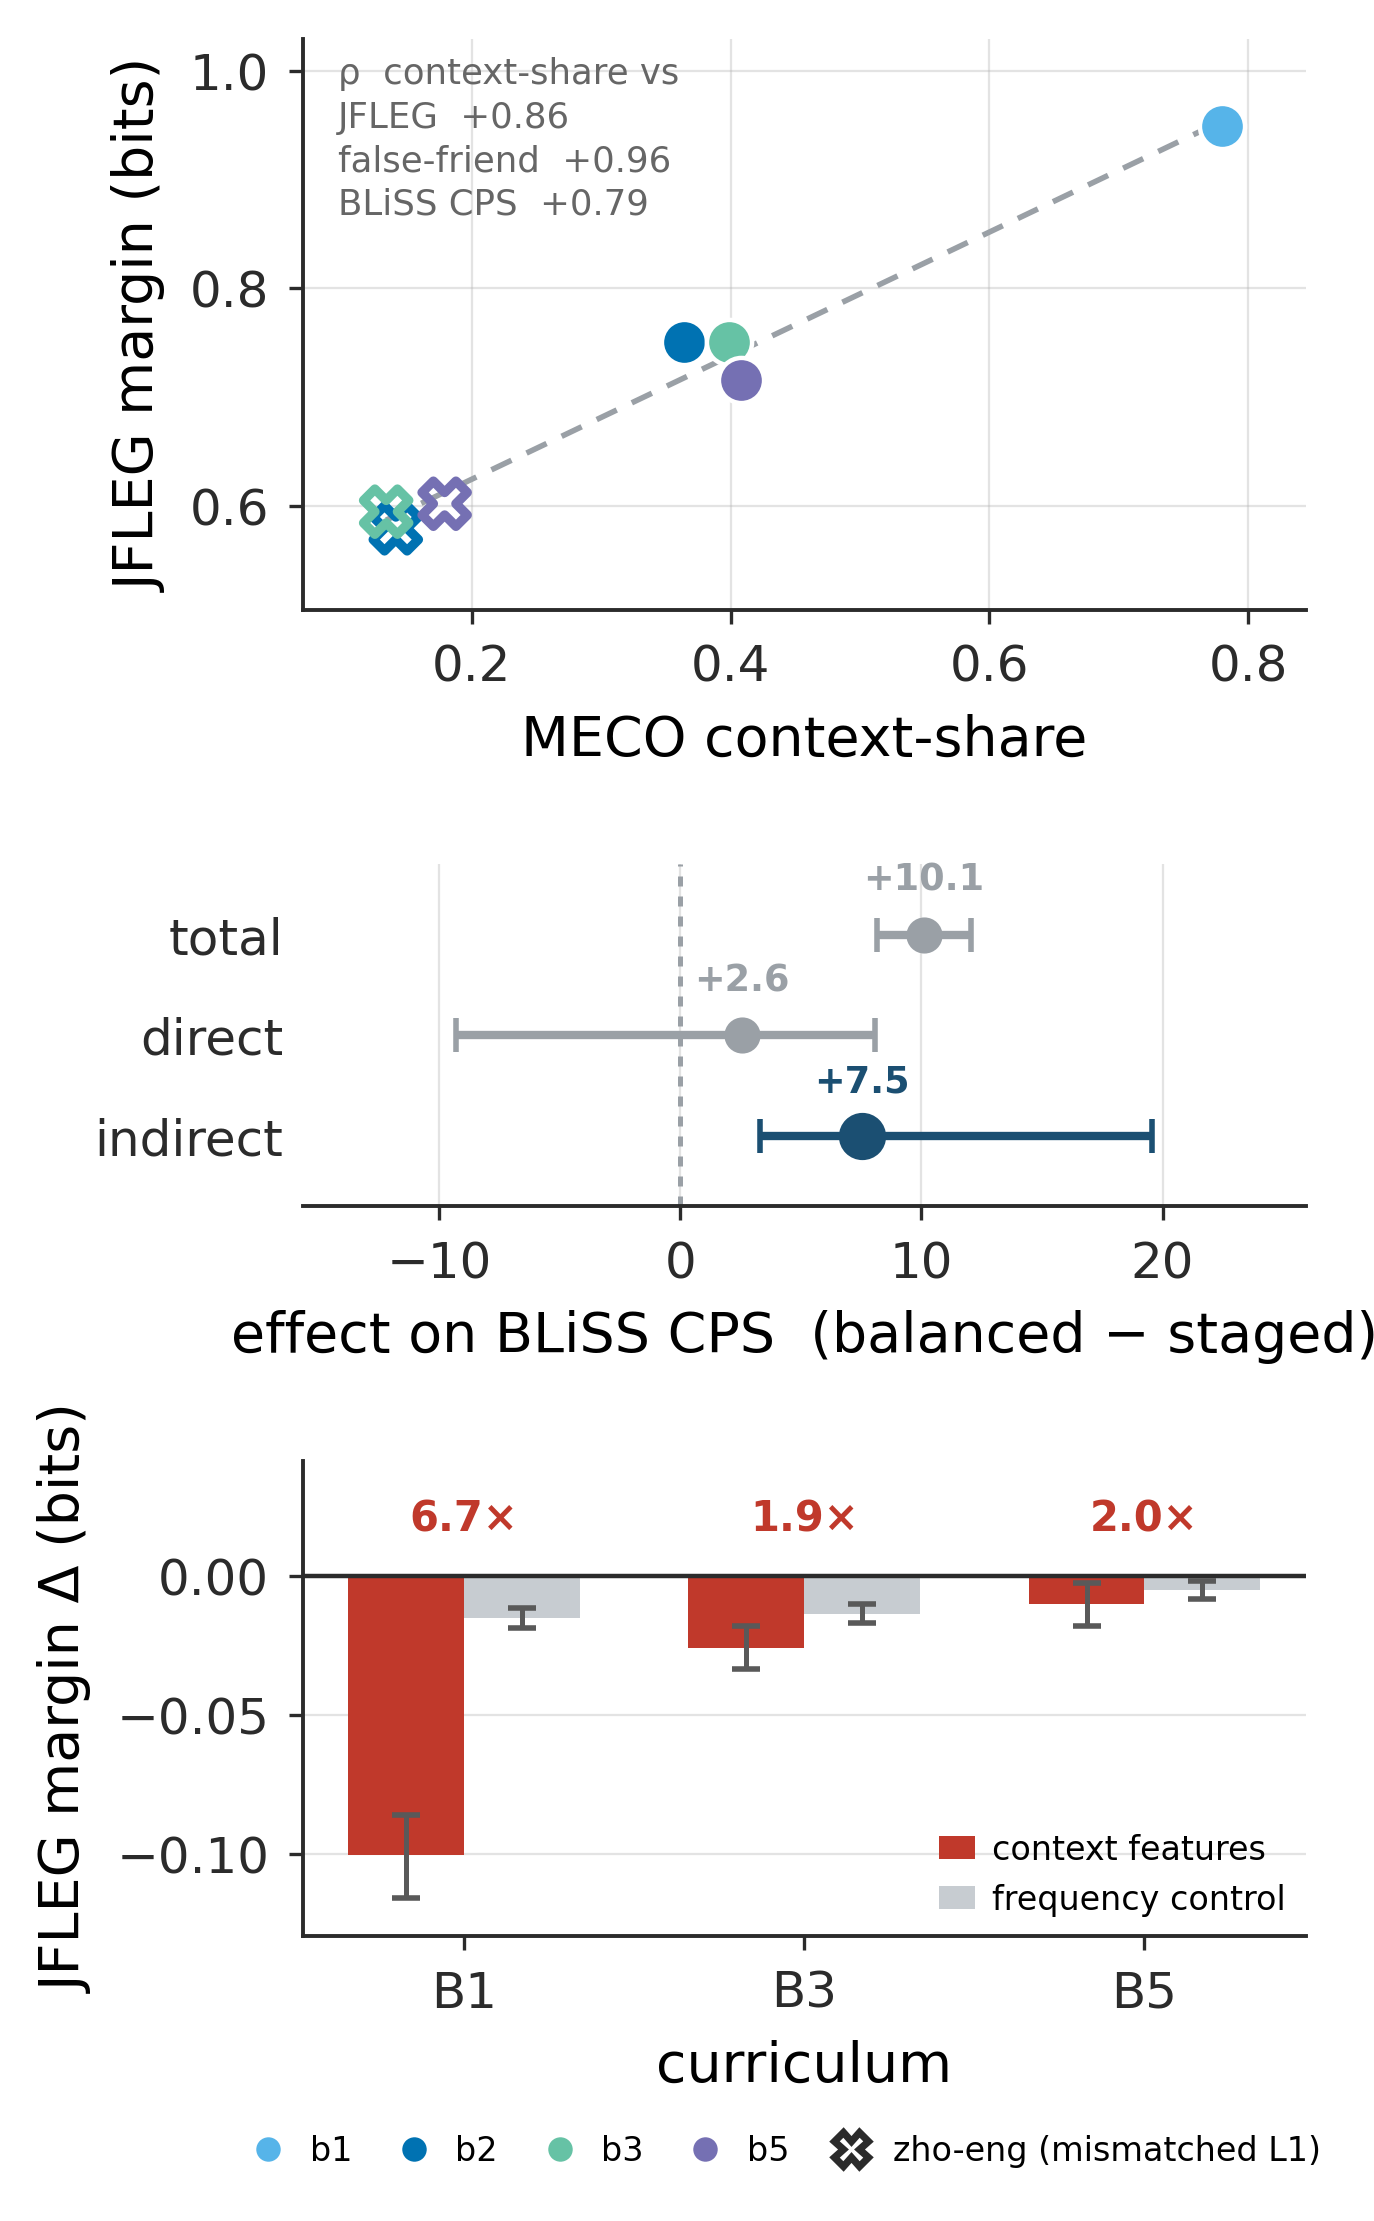
\includegraphics[width=\columnwidth]{fig/fig_single_axis_combined.png}
  \caption{\textbf{Within-model SAE ablation (JFLEG, exploratory).} Zeroing the top-50 context-share SAE features degrades the JFLEG learner-fluency margin $1.9$--$6.7\times$ more than a matched frequency-feature control (context CIs exclude zero); the parallel BLiSS-CPS arm is null. Layer~8, FineWeb-2B nld--eng, single model; associational, not causal.}
  \label{fig:single-axis}
\end{figure}
 
\subsection{Canonical results tables}\label{sec:meco-canonical-app}
 
Tab.~\ref{tab:meco} is the compact canonical summary; the complete per-language and per-condition results are given in Tabs.~\ref{tab:meco_langrows}--\ref{tab:meco_full_canonical}. All cells are single-seed point estimates of Eq.~\ref{eq:meco-spec}; uncertainty is addressed in \S\ref{sec:sig-uncertainty}. The primary curriculum comparisons use only the \emph{matched diagonal} --- each L1$\to$English model scored on its own L1 reader group (nld$\to$Dutch, deu$\to$German, zho$\to$Chinese) --- whose $\Delta\log L$ values sit in a bounded, mutually comparable range and are reproducible under re-scoring. The incomplete-within-language-standardisation pathology is confined to \emph{off-diagonal} cross-L1 cells (an L1 model scored on a different reader cluster; the $\dagger$ rows in Tab.~\ref{tab:meco_full_canonical}), which we do not embolden and never treat as evidence.
 
\begin{table}[!ht]
  \centering
  \small
  \caption{Aggregated MECO~L2 $\Delta\log L$ summary value (mean over reader-L1s within each L2 language). Bold marks the largest value per L2 language; the LLM rows are \emph{contextual only} (tokeniser, architecture, and subword aggregation differ, so no cross-class ranking is intended). The strongest cross-class comparator, Baichuan-7B, slightly exceeds \beetle{} on German.}
  \label{tab:meco}
  \begin{tabular}{lrrr}
    \toprule
    Model & Dutch L2 & German L2 & Chinese L2 \\
    \midrule
    BLOOM-1b1 (best legacy) & 41.5 & 179.7 & \textbf{164.3} \\
    BLOOM-7b1               & 19.7 & 115.9 & 84.7 \\
    XGLM-4.5B               & 8.7  & 19.0  & 22.6 \\
    Baichuan-7B (best modern) & 88.3 & \textbf{185.1} & 31.2 \\
    \beetle{} best (per cell) & \textbf{139.6} & 184.7 & 115.4 \\
    \beetle{} canonical mean & 81.1 & 167.0 & 130.4 \\
    modern-bilingual aggr.\ mean & 12.3 & 97.5 & 56.3 \\
    \bottomrule
  \end{tabular}
\end{table}
 
 
% =====================================================================
\section{Statistical Significance Testing}\label{sec:significance-comprehensive}
 
This section reports the inferential analyses underlying the claims in the main text. The analysis code and the corresponding result files are released alongside the paper. The within-seed cross-cohort associations are in \S\ref{sec:sig-core}; the between-seed inferential anchor and robustness tests follow in \S\ref{sec:sig-robustness}; all uncertainty caveats and the family-correction policy are in \S\ref{sec:sig-uncertainty}.
 
\subsection{Within-seed cross-cohort associations}\label{sec:sig-core}
 
Three tests carry the cross-cohort and curriculum comparisons. They are computed across cells and observations \emph{within} single seeds, so the large $d$ and small $p$ reflect within-seed cell counts, not between-seed replication. We treat them as descriptive cross-cohort associations; the inferential weight for the curriculum claim rests on the between-seed ablation (\S\ref{sec:sig-robustness}).
 
\paragraph{(1) Fisher $z$-test on coupling magnitude.} We test whether the set of \beetle{} bilingual models exhibits higher MECO~$\rho$ than each baseline class, with \beetle{} as reference ($n=512$ cells) and FDR-corrected two-sided $p$ (Tab.~\ref{tab:sig_fisher}). Every comparison is highly significant with very large effect sizes (Cohen's $d\in[6.6,13.8]$).
 
\begin{table}[!ht]
  \centering \small
  \caption{\textbf{Fisher $z$-test, \beetle{} bilingual reference vs.\ each baseline class (contextual).} A within-seed cross-cell association, not a between-seed or cross-class ranking. $n_\textsc{ref}=512$ cells; $p$ two-sided, FDR-corrected; $d$ on $z$-transformed $\rho$.}
  \label{tab:sig_fisher}
  \begin{tabular}{lrrrr}
    \toprule
    Comparator & $\bar\rho_\textsc{ref}$ & $\bar\rho_\textsc{other}$ & $d$ & $p$ \\
    \midrule
    B-GPT           & 0.975 & 0.954 & 6.59  & $2.8{\times}10^{-29}$ \\
    bilingual LLMs  & 0.975 & 0.935 & 10.30 & $1.8{\times}10^{-6}$ \\
    BLOOM-ladder    & 0.975 & 0.911 & 13.79 & $1.5{\times}10^{-12}$ \\
    EuroLLM         & 0.975 & 0.937 & 9.93  & $6.7{\times}10^{-8}$ \\
    \bottomrule
  \end{tabular}
\end{table}
 
\paragraph{(2) Mixed-effects surprisal $\times$ model\_type interaction.} A linear mixed-effects model with subject and sentence random intercepts and a fixed-effect surprisal-by-model-class interaction (Tab.~\ref{tab:sig_mixedlm_baselines}). Every baseline class shows a \emph{negative} interaction with $z$-surprisal --- it loses per-bit reading-time coupling relative to the \beetle{} reference --- with the BLOOM ladder losing the most ($\beta=-0.085$, $p<10^{-154}$).
 
\begin{table}[!ht]
  \centering \small
  \caption{\textbf{Baseline-anchored mixed-effects fit (contextual)} (\beetle{} bilingual = reference). A within-seed cross-cell association, not a cross-class ranking.}
  \label{tab:sig_mixedlm_baselines}
  \begin{tabular}{lrrr}
    \toprule
    Term & $\beta$ & SE & $p$ \\
    \midrule
    $z$-surprisal                          & $+0.464$ & 0.0017 & $<10^{-300}$ \\
    \quad $\times$ bilingual\_llm          & $-0.037$ & 0.0041 & $1.6{\times}10^{-19}$ \\
    \quad $\times$ bloom\_ladder           & $-0.085$ & 0.0032 & $4.0{\times}10^{-155}$ \\
    \quad $\times$ eurollm                 & $-0.038$ & 0.0036 & $9.0{\times}10^{-26}$ \\
    \quad $\times$ small\_bilingual        & $+0.063$ & 0.0017 & $3.5{\times}10^{-288}$ \\
    \bottomrule
  \end{tabular}
\end{table}
 
\paragraph{(3) Curriculum $\times$ eye-measure interaction.} The early-vs-late eye-measure pattern of \S\ref{sec:meco-stage-app} is backed by a peak-encoding depth test (Tab.~\ref{tab:sig_decomp_dissociation}): staged curricula peak at deeper layers than balanced for both measure bands, with the larger gap in the early band.
 
\begin{table}[!ht]
  \centering \small
  \caption{\textbf{Peak-encoding depth dissociation, balanced vs.\ staged.} Mann--Whitney on per-fit normalised peak layer depth (0=embedding, 1=output).}
  \label{tab:sig_decomp_dissociation}
  \begin{tabular}{lrrrr}
    \toprule
    Stage & $\overline{\text{peakfrac}}_\textsc{bal}$ & $\overline{\text{peakfrac}}_\textsc{stg}$ & $U$ & $p$ \\
    \midrule
    early (first-fix / first-run) & 0.702 & 0.809 & 6767.0 & $5.4{\times}10^{-6}$ \\
    late (refixation / regression) & 0.762 & 0.820 & 8055.5 & $5.5{\times}10^{-3}$ \\
    \bottomrule
  \end{tabular}
\end{table}
 
\subsection{Between-seed anchor and robustness tests}\label{sec:sig-robustness}
 
\paragraph{Within-family ablation (between-seed anchor).} The B1/B2/B3 ablation families are decided on the MECO Spearman~$\rho$ between per-subject $\beta$-surprisal and reading time using a paired permutation test on $n=3$ pre-registered seeds $\{13,42,97\}$ per variant, Holm-corrected within family at $\alpha{=}0.05$. \emph{No family declares a winner at $\alpha{=}0.05$ on the three-seed set} (Tabs.~\ref{tab:sig_B1}--\ref{tab:sig_B3}): the largest effects are $d_z=1.39$ (B1 vs.\ B1b), $1.63$ (B2 vs.\ B2-lr), and $-0.63$ (B3 vs.\ B3-full), but small $n$ keeps $p_{\mathrm{holm}}$ above threshold. This is why the body treats B2/B3/B5 as a class rather than naming a single variant.
 
\begin{table}[!ht]
  \centering \small
  \caption{\textbf{B1 / B3 family ablations (single pair each).} Paired permutation on MECO~$\rho$, $n=3$ seeds; Holm-corrected within family.}
  \label{tab:sig_B1}
  \begin{tabular}{lrrrr}
    \toprule
    Pair & $\bar\rho_a$ & $\bar\rho_b$ & $d_z$ & $p_{\mathrm{holm}}$ \\
    \midrule
    B1 vs.\ B1b     & 0.336 & 0.246 & $+1.386$ & 0.250 \\
    B3 vs.\ B3-full & 0.201 & 0.288 & $-0.631$ & 0.500 \\
    \bottomrule
  \end{tabular}
\end{table}
 
\begin{table}[!ht]
  \centering \small
  \caption{\textbf{B2 family ablation (continual-learning overlays).} Paired permutation on MECO~$\rho$, $n=3$ seeds; Holm-corrected over six pairs. No overlay survives Holm at $\alpha{=}0.05$.}
  \label{tab:sig_B3}
  \begin{tabular}{lrrrr}
    \toprule
    Pair & $\bar\rho_a$ & $\bar\rho_b$ & $d_z$ & $p_{\mathrm{holm}}$ \\
    \midrule
    B2 \,vs.\ B2-ewc      & 0.309 & 0.294 & $+0.155$ & 1.000 \\
    B2 \,vs.\ B2-lamol    & 0.309 & 0.307 & $+0.039$ & 1.000 \\
    B2 \,vs.\ B2-lr       & 0.309 & 0.173 & $+1.624$ & 1.000 \\
    B2-ewc vs.\ B2-lamol  & 0.294 & 0.307 & $-0.079$ & 1.000 \\
    B2-ewc vs.\ B2-lr     & 0.294 & 0.173 & $+0.954$ & 1.000 \\
    B2-lamol vs.\ B2-lr   & 0.307 & 0.173 & $+1.634$ & 1.000 \\
    \bottomrule
  \end{tabular}
\end{table}
 
\paragraph{Decomposition tests (model level, canonical).} The decomposition backing \S\ref{sec:meco-mech-app} is computed at the model level (one value per model, label-permutation over models, ablations excluded), the unit that avoids the pseudo-replication of per-fit pooling. Balanced models carry a larger long-context share than staged at FineWeb-100M ($0.43$ vs.\ $0.09$, $\Delta{=}{+}0.34$, $p_\text{perm}{<}10^{-4}$) and pooled across scales ($\Delta{=}{+}0.24$, $p_\text{perm}{<}10^{-4}$), with the mirror split on the frequency share ($\Delta{=}{-}0.36$, $p_\text{perm}{=}6{\times}10^{-5}$ at 100M) and no difference on the local share ($p_\text{perm}{=}0.66$). A scale-pooled per-fit Mann--Whitney on ($\Delta\log L_\textsc{long}-\Delta\log L_\textsc{local}$) agrees descriptively ($U{=}7048.0$, $p{=}4.1{\times}10^{-3}$). The per-scale and pooled model-level contrasts are in Tab.~\ref{tab:sig_decomp_curriculum}.
 
\begin{table}[!ht]
  \centering \small
  \caption{\textbf{Balanced vs.\ staged decomposition share, model level.} One value per model (mean over the three MECO languages), continual-learning ablations excluded. Staged curricula carry far less long-context share and a correspondingly larger frequency share; the local component is shared (model-level $p_\text{perm}{=}0.66$ at 100M, $0.27$ pooled). Superscripts are model-level label-permutation $p$ over models.}
  \label{tab:sig_decomp_curriculum}
  \begin{tabular}{llcccc}
    \toprule
     & & \multicolumn{2}{c}{Long-context share} & \multicolumn{2}{c}{Frequency share} \\
    \cmidrule(lr){3-4}\cmidrule(lr){5-6}
    Regime & $n_{\text{bal}}/n_{\text{stg}}$ & Bal. & Staged & Bal. & Staged \\
    \midrule
    FineWeb-100M & 9/18 & 0.43 & 0.09${}^{<10^{-4}}$ & 0.10 & 0.47${}^{6.0\times10^{-5}}$ \\
    FineWeb-2B & 4/12 & 0.36 & 0.16${}^{0.010}$ & 0.17 & 0.36${}^{0.054}$ \\
    FineWeb-24B & 5/11 & 0.56 & 0.41${}^{0.080}$ & 0.04 & 0.11${}^{0.021}$ \\
    Pooled & 20/51 & 0.43 & 0.18${}^{<10^{-4}}$ & 0.12 & 0.41${}^{2.0\times10^{-5}}$ \\
    \bottomrule
  \end{tabular}
\end{table}
 
\paragraph{Omnibus and pairwise tests.} The Friedman omnibus confirms a positive surprisal--reading-time relation within each language band (Tab.~\ref{tab:sig_friedman}), and the pairwise Wilcoxon comparison finds $2{,}159$ baseline-vs-\beetle{} comparisons significant at Holm-corrected $p<0.05$ with zero within-\beetle{} pairs rejecting (Tab.~\ref{tab:sig_wilcoxon_examples}) --- the cross-cohort gap is uniformly significant while within-\beetle{} single-seed curriculum differences are not separable from noise.
 
\begin{table}[!ht]
  \centering \small
  \caption{\textbf{Friedman $\chi^2$ on $\mathbb{I}[\rho>0]$ across languages} (FDR-corrected). Both English- and Dutch-reader bands reject at $p<10^{-43}$.}
  \label{tab:sig_friedman}
  \begin{tabular}{llrr}
    \toprule
    Cohort & Reader language & $n_\textsc{models}$ & $p_\textsc{fdr}$ \\
    \midrule
    \beetle{} bilingual & English & 256 & $4.8{\times}10^{-44}$ \\
    \beetle{} bilingual & Dutch   & 256 & $4.8{\times}10^{-44}$ \\
    Baselines           & English & 284 & $1.3{\times}10^{-48}$ \\
    Baselines           & Dutch   & 284 & $1.3{\times}10^{-48}$ \\
    \bottomrule
  \end{tabular}
\end{table}
 
\begin{table}[!ht]
  \centering \small
  \caption{\textbf{Pairwise Wilcoxon signed-rank examples} on MECO sentence-level reading-time error (Holm-corrected). \beetle{} has strictly lower mean error than each BLOOM cell; every example rejects at $p_\textsc{holm}<10^{-3}$.}
  \label{tab:sig_wilcoxon_examples}
  \begin{tabular}{llrrr}
    \toprule
    Model $a$ & Model $b$ & $W$ & $p_\text{raw}$ & $p_\textsc{holm}$ \\
    \midrule
    \beetle{} nld mono & BLOOM-560m & 12 & $1.3{\times}10^{-10}$ & $5.1{\times}10^{-6}$ \\
    \beetle{} nld mono & BLOOM-1b1  & 22 & $9.7{\times}10^{-10}$ & $3.8{\times}10^{-5}$ \\
    \beetle{} nld mono & BLOOM-1b7  & 41 & $1.8{\times}10^{-8}$  & $7.1{\times}10^{-4}$ \\
    \beetle{} nld mono & BLOOM-3b   & 21 & $8.1{\times}10^{-10}$ & $3.2{\times}10^{-5}$ \\
    \beetle{} nld mono & BLOOM-7b1  & 32 & $5.0{\times}10^{-9}$  & $2.0{\times}10^{-4}$ \\
    \bottomrule
  \end{tabular}
\end{table}
 
\paragraph{BLiSS per-cell binomials.} Benjamini--Hochberg FDR-corrected across the matched-L1 per-CEFR $\times$ 4-metric family (final checkpoint, B1--B5; $217$ cells, $868$ tests), $216/868$ ($25\%$) reject at $q<0.05$. The survivors match the raw pattern: RP$@0$ ($60/217$ cells) and NGS ($69/217$) rejections are uniformly above chance, whereas CPS rejections are overwhelmingly \emph{below} chance ($69$ of $72$), confirming the CPS inversion under L2 schedules; RP$@\tau$ is weak ($15/217$, split in direction).
 
\subsection{Caveats and family-correction policy}\label{sec:sig-uncertainty}
 
\paragraph{Single-seed point estimates.} Except where a seed grid is explicitly named, every MECO and BLiSS cell in this appendix is a single-seed point estimate. We do not report per-cell within-fit bootstrap CIs because, at one seed per cell, the within-fit CI is not what discriminates between curricula; the relevant variance is between-seed.
 
\paragraph{Per-seed $\Delta\log L$ (three seeds).} Re-scoring the released B3-33 nld--eng HS checkpoint through the canonical procedure returns Dutch-reader $\Delta\log L = 139.8$, matching the reported $139.6$, so the principal result is reproducible under re-evaluation. A set of three seeds ($\{13,42,97\}$) scored through the same procedure gives small within-configuration between-seed variance (B1 $\sigma{=}3.7$, B2 $11.3$, B3-33 $5.9$) and reproduces the principal B3-33-over-B1 advantage (B3-33 mean $83.3 >$ B1 $77.6$); the higher-variance B2 condition ($74.9$) falls just below B1 here, reversing the order of the closely spaced B1 and B2 conditions. This set of runs sits at a lower absolute level (a reduced single-GPU training configuration), so it corroborates the \emph{direction} rather than the magnitude.
 
\paragraph{Evidentiary tiers.} The \emph{primary} curriculum measure is $\Delta\log L$ on \texttt{firstrun.dur} (\S\ref{sec:meco-headline-app}), backed by the three core tests of \S\ref{sec:sig-core} and the between-seed ablation of \S\ref{sec:sig-robustness}. The likelihood decomposition's context-share split (\S\ref{sec:meco-mech-app}, Tab.~\ref{tab:sig_decomp_curriculum}) is a \emph{secondary} model-level result. The within-model SAE ablation and the cross-task context-share correlations remain \emph{exploratory} (single-model/single-task or $n{=}8$).
 
\paragraph{Family-correction policy.} Corrections are applied per family: within-family Holm for the ablation pairs and the pairwise Wilcoxon comparison; Benjamini--Hochberg FDR for the Fisher~$z$ cross-class comparisons, the Friedman omnibus, and the per-cell BLiSS binomials; and uncorrected permutation / Mann--Whitney for the decomposition tests, a small logically-coherent family for which correction is uninformative. No body claim relies on uncorrected $p$-values from a multi-test family.
 
 
% ####################################################################
% ===== BLOCK H --- ROBUSTNESS, HIERARCHICAL RECONCILIATION & SUPPLEMENTARY TABLES =====
% ####################################################################
% =====================================================================
\section{Hierarchical Model of Structured Variation}\label{sec:hier-model}
 
\paragraph{Motivation.} The matched-L1 curriculum comparison (Tab.~\ref{tab:meco_curriculum_matched}) is an unbalanced grid: each cell is a single curriculum$\times$L1$\times$scale configuration with one seed. Comparing cells in isolation conflates the curriculum effect with L1 baseline differences (Chinese readers sit far above Germanic ones), with scale, and with measurement noise. We fit a \textbf{hierarchical model} that treats every observed score as arising from one generative process with structured sources of variation, applies partial pooling so cells borrow strength, and yields probability statements rather than bare point estimates. We report a frequentist mixed model (\texttt{statsmodels}~\citep{seabold2010statsmodels}) and a Bayesian fit (\texttt{bambi}/\texttt{PyMC}~\citep{capretto2022bambi,abrilpla2023pymc}, summarised with \texttt{ArviZ}~\citep{kumar2019arviz}); the design follows standard multilevel practice~\citep{gelman2007data}.
 
\paragraph{Specification.} Let $y_{c,l,s}$ be the MECO~$\Delta\log L$ of the model with curriculum $c\in\{$B1$,\dots,$B5$\}$, training L1 $l$, at scale $s$, on its matched reader population. The principal model (M1) is, in Wilkinson notation,
\begin{equation}
y_{c,l,s} \sim \mathrm{curriculum}\,*\,\mathrm{scale} \;+\; (1 \mid \mathrm{L1}),
\label{eq:hier-m1}
\end{equation}
with $b_l\sim\mathcal{N}(0,\sigma^2_{\mathrm{L1}})$ and B1, HumanScale-100M as reference levels. To attribute variance we fit a components model (M2) adding $(1\mid\mathrm{scale})$ and $(1\mid\mathrm{curriculum{:}L1})$, and on the reduced seed grid a seed-variance model (M3) $y\sim\mathrm{curriculum}+(1\mid\mathrm{seed})$. Bayesian fits use weakly-informative priors, 4 chains $\times$ 1500 post-warmup draws, \texttt{target\_accept}${=}0.95$. We report $P(\cdot)$, the probability a contrast is positive (Bayesian posterior, or a hierarchical bootstrap resampling L1 clusters where the Bayesian fit is unavailable).
 
\paragraph{Where the variation lives.} The decomposition (Tab.~\ref{tab:hier-varcomp}, Fig.~\ref{fig:hier-varcomp-forest}) attributes most $\Delta\log L$ variance to differences \emph{between L1s} ($\hierVarLone\%$) and within-cell residual ($\hierVarResid\%$), with scale at $\hierVarScale\%$ and curriculum$\times$L1 at $\hierVarCurrLone\%$; the curriculum main effect is a smaller share ($\hierVarCurr\%$) precisely because its sign is consistent while its magnitude is L1- and scale-modulated. Extending to the matched L1 families on the $\beta$(surprisal) axis (FineWeb-100M) corroborates this: across six matched L1s (Germanic, Romance, Slavic, Turkic, Sinitic) the pooled staged-over-balanced advantage is positive ($\Delta\beta=+5.3$, $95\%$ hierarchical-bootstrap CI over L1 clusters $[+2.2,+8.5]$, $P{>}0.99$; Fig.~\ref{fig:l1_generality}), with the curriculum main effect ($10.8\%$ of $\beta$ variance) and curriculum$\times$L1 interaction ($9.0\%$) comparable --- real but L1-modulated.
 
\begin{table}[ht]
  \centering \small
  \setlength{\tabcolsep}{5pt}
  \caption{\textbf{Variance decomposition of MECO~$\Delta\log L$} over the matched curriculum$\times$L1$\times$scale cube ($n{=}\hierNrows$ cells, $\hierNLone$ matched L1s; ANOVA share, cross-checked by the Bayesian variance components). The curriculum effect is modulated by L1 and scale rather than constituting a large standalone main effect.}
  \label{tab:hier-varcomp}
  \begin{tabular}{lr}
    \toprule
    Source & Variance share \\
    \midrule
    Curriculum                 & $\hierVarCurr\%$ \\
    Scale / cohort             & $\hierVarScale\%$ \\
    L1                         & $\hierVarLone\%$ \\
    Curriculum $\times$ L1     & $\hierVarCurrLone\%$ \\
    Residual                   & $\hierVarResid\%$ \\
    \midrule
    \multicolumn{2}{l}{\textit{Noise scales}} \\
    Within-config seed $\sigma_{\mathrm{seed}}$ & $\hierSigmaSeed$ \\
    Residual $\sigma$ (M1)     & $\hierSigmaResid$ \\
    \bottomrule
  \end{tabular}
\end{table}
 
\paragraph{Curriculum contrasts.} Table~\ref{tab:hier-contrasts} reports curriculum-vs-B1 contrasts at each scale with $P(\text{contrast}{>}0)$. The staged-over-balanced advantage is large and decisive at HumanScale-100M (B3$-$B1${=}\hierDBthreeBoneHS$, $P{=}\hierPBthreeBoneHS$; B5$-$B1 $P{=}\hierPBfiveBoneHS$), behaves \emph{non-monotonically} in scale --- diminishing to a negligible level at FineWeb-2B (B3$-$B1${=}\hierDBthreeBoneFWtwoB$, $P{=}\hierPBthreeBoneFWtwoB$, where the Chinese reversal cancels the Germanic gains) and recovering to a positive but wide estimate at FineWeb-24B (B3$-$B1${=}\hierDBthreeBoneFWtfB$, $P{=}\hierPBthreeBoneFWtfB$) --- and remains positive pooled across scales (B3$-$B1${=}\hierDBthreeBonePooled$, $P{=}\hierPBthreeBonePooled$).
 
\begin{table}[ht]
  \centering \small
  \setlength{\tabcolsep}{4pt}
  \caption{\textbf{Curriculum contrasts vs.\ B1 on MECO~$\Delta\log L$} (released checkpoints), as $\Delta\log L$ point estimate with $P(\text{contrast}{>}0)$ in parentheses. Staged schedules exceed balanced decisively at the smallest scale; the contrast is non-monotonic in scale and positive when pooled.}
  \label{tab:hier-contrasts}
  \begin{tabular}{lcccc}
    \toprule
    & HS-100M & FW-2B & FW-24B & Pooled \\
    \midrule
    B2$-$B1 & $\hierDBtwoBoneHS$ ($\hierPBtwoBoneHS$) & $\hierDBtwoBoneFWtwoB$ ($\hierPBtwoBoneFWtwoB$) & $\hierDBtwoBoneFWtfB$ ($\hierPBtwoBoneFWtfB$) & $\hierDBtwoBonePooled$ ($\hierPBtwoBonePooled$) \\
    B3$-$B1 & $\hierDBthreeBoneHS$ ($\hierPBthreeBoneHS$) & $\hierDBthreeBoneFWtwoB$ ($\hierPBthreeBoneFWtwoB$) & $\hierDBthreeBoneFWtfB$ ($\hierPBthreeBoneFWtfB$) & $\hierDBthreeBonePooled$ ($\hierPBthreeBonePooled$) \\
    B5$-$B1 & $\hierDBfiveBoneHS$ ($\hierPBfiveBoneHS$) & $\hierDBfiveBoneFWtwoB$ ($\hierPBfiveBoneFWtwoB$) & $\hierDBfiveBoneFWtfB$ ($\hierPBfiveBoneFWtfB$) & $\hierDBfiveBonePooled$ ($\hierPBfiveBonePooled$) \\
    \bottomrule
  \end{tabular}
\end{table}
 
\begin{figure*}[ht]
  \centering
  \begin{subfigure}{0.66\textwidth}
    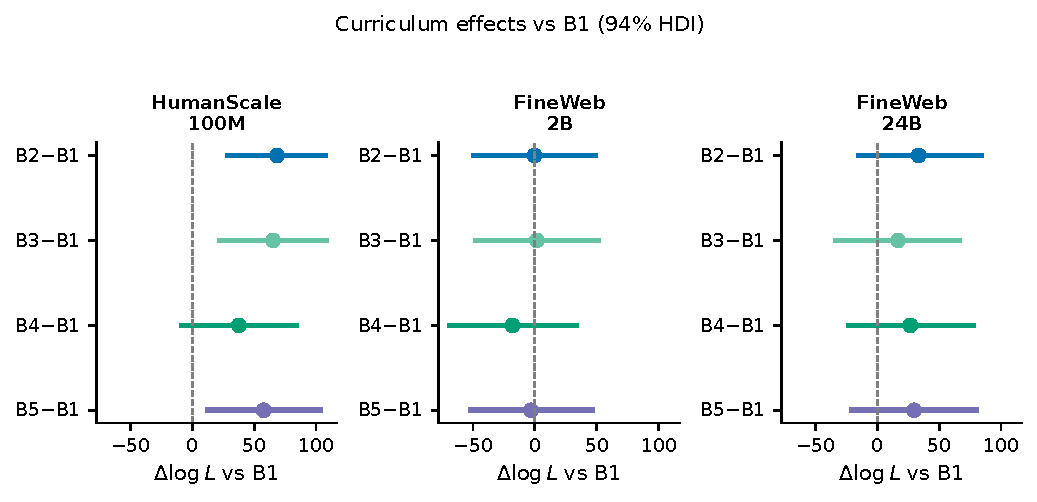
\includegraphics[width=\linewidth]{fig/hier/fig_hier_forest.pdf}
    \caption{Curriculum effects vs.\ B1 by scale (point estimate $\pm$ interval).}
    \label{fig:hier-forest}
  \end{subfigure}\hfill
  \begin{subfigure}{0.32\textwidth}
    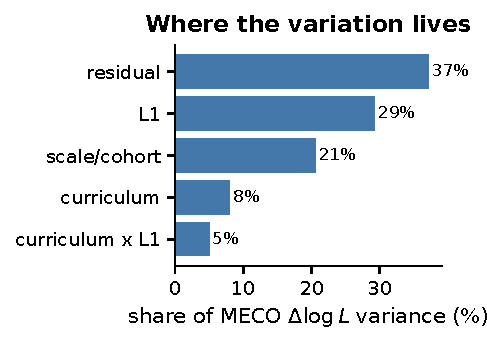
\includegraphics[width=\linewidth]{fig/hier/fig_hier_varcomp.pdf}
    \caption{Variance decomposition.}
    \label{fig:hier-varcomp}
  \end{subfigure}
  \caption{\textbf{Hierarchical analysis of MECO~$\Delta\log L$.} (\subref{fig:hier-forest})~Staged-over-balanced contrasts are large and positive at HumanScale-100M, near zero at FineWeb-2B, and positive but wide at FineWeb-24B. (\subref{fig:hier-varcomp})~Most variance is between-L1 and residual; curriculum and curriculum$\times$L1 are smaller, modulated shares.}
  \label{fig:hier-varcomp-forest}
\end{figure*}
 
\paragraph{Seeds.} On the canonically-scored three-seed grid (B1/B2/B3-33 nld--eng, HumanScale-100M), within-configuration seed spread is small ($\sigma_{\mathrm{seed}}{=}\hierSigmaSeed~\Delta\log L$), confirming seed noise \emph{per se} is minor. The grid preserves the B3-33-over-B1 lead but swaps the closely-spaced B1/B2 pair (B1 edges B2 here), so it corroborates the B3-over-B1 \emph{direction} without establishing strict ranking stability among the staged curricula.
 
\paragraph{Caveats.} Only $\hierNLone$ training L1s are matched to MECO reader populations, so $\sigma_{\mathrm{L1}}$ is weakly identified and reported from the regularised Bayesian posterior; the six-L1 $\beta$ decomposition gives a complementary, better-identified view. Seeds are replicated in a single sub-cube. The released cube is small ($n{=}\hierNrows$), so several intervals are wide --- we report $P(\cdot)$ rather than claiming significance, and treat contrasts near $P{=}0.5$ as undetermined.
 
 
% =====================================================================
\section{MECO Supplementary Tables}\label{sec:supp-tables}
 
\begin{table*}[!ht]
  \centering \small
  \caption{\textbf{Canonical per-language MECO~L2 rows.} Per (model, L2-language) cell on the wave-1$+$wave-2 joined data: $\log L$ of the full model, of the baseline, and $\Delta\log L$. Larger $\Delta\log L$ indicates better surprisal alignment. $^{\dagger}$ Cross-L1 cells (the \texttt{nl-en} B-GPT model scored on the German and Chinese reader clusters, $243.00$ and $221.61$, both far above its matched Dutch cell $88.25$) can be inflated by incomplete within-language standardisation and are not used as primary evidence; see Tab.~\ref{tab:meco_full_canonical}.}
  \label{tab:meco_langrows}
  \begin{tabular}{lrrrl}
    \toprule
    Model & $\log L$ & Baseline $\log L$ & $\Delta\log L$ & Class \\
    \midrule
    \multicolumn{5}{l}{\textit{Dutch (\texttt{nld})}} \\
    \midrule
    B-GPT nl-en simul. & $-193987.48$ & $-194075.73$ & $88.25$ & B-GPT \\
    XGLM-4.5b & $-194066.67$ & $-194075.32$ & $8.65$ & XGLM \\
    BLOOM-1b1 & $-194033.84$ & $-194075.32$ & $41.47$ & BLOOM \\
    BLOOM-1b7 & $-194040.91$ & $-194075.32$ & $34.41$ & BLOOM \\
    BLOOM-560m & $-194031.03$ & $-194075.32$ & $44.29$ & BLOOM \\
    BLOOM-7b1 & $-194055.62$ & $-194075.32$ & $19.69$ & BLOOM \\
    mono-nld & $-193979.29$ & $-194075.32$ & $96.02$ & mono-NLD \\
    mono-eng & $-194010.19$ & $-194075.32$ & $65.13$ & mono-ENG \\
    B1 nld-eng HS & $-194012.99$ & $-194075.32$ & $62.33$ & L2 bal. \\
    B2 nld-eng HS & $-193940.18$ & $-194075.32$ & $135.14$ & L2 sim. \\
    B3-0 nld-eng HS & $-193936.56$ & $-194075.32$ & $138.75$ & L2 seq. \\
    B3-33 nld-eng HS & $-193935.73$ & $-194075.32$ & $139.58$ & L2 seq. \\
    B4 nld-eng HS & $-193953.55$ & $-194075.32$ & $121.77$ & L2 class. \\
    B5 nld-eng HS & $-193937.57$ & $-194075.32$ & $137.74$ & L2 late \\
    \midrule
    \multicolumn{5}{l}{\textit{Chinese (\texttt{zho})}} \\
    \midrule
    B-GPT nl-en simul. & $-233899.84$ & $-234121.45$ & $221.61^{\dagger}$ & B-GPT \\
    BLOOM-1b1 & $-233957.22$ & $-234121.53$ & $164.30$ & BLOOM \\
    BLOOM-7b1 & $-234036.80$ & $-234121.53$ & $84.73$ & BLOOM \\
    mono-zho & $-234116.14$ & $-234121.53$ & $5.39$ & mono-ZHO \\
    B1 zho-eng HS & $-234015.83$ & $-234121.53$ & $105.69$ & L2 bal. \\
    B2 zho-eng HS & $-234021.38$ & $-234121.53$ & $100.14$ & L2 sim. \\
    B3-33 zho-eng HS & $-234018.37$ & $-234121.53$ & $103.15$ & L2 seq. \\
    B4 zho-eng HS & $-234022.81$ & $-234121.53$ & $98.71$ & L2 class. \\
    B5 zho-eng HS & $-234006.13$ & $-234121.53$ & $115.40$ & L2 late \\
    \midrule
    \multicolumn{5}{l}{\textit{German (\texttt{deu})}} \\
    \midrule
    B-GPT nl-en simul. & $-275130.72$ & $-275373.70$ & $243.00^{\dagger}$ & B-GPT \\
    BLOOM-1b1 & $-275193.91$ & $-275373.57$ & $179.66$ & BLOOM \\
    BLOOM-7b1 & $-275257.67$ & $-275373.57$ & $115.90$ & BLOOM \\
    mono-deu & $-275239.27$ & $-275373.57$ & $134.29$ & mono-DEU \\
    B1 deu-eng HS & $-275298.46$ & $-275373.57$ & $75.10$ & L2 bal. \\
    B2 deu-eng FW & $-275188.90$ & $-275373.57$ & $184.66$ & L2 sim. \\
    B2 deu-eng HS & $-275207.30$ & $-275373.57$ & $166.27$ & L2 sim. \\
    B3-33 deu-eng HS & $-275196.11$ & $-275373.57$ & $177.45$ & L2 seq. \\
    B4 deu-eng HS & $-275233.00$ & $-275373.57$ & $140.57$ & L2 class. \\
    B5 deu-eng HS & $-275205.21$ & $-275373.57$ & $168.36$ & L2 late \\
    \bottomrule
  \end{tabular}
\end{table*}
 
\begin{table*}[!ht]
  \centering \scriptsize
  \setlength{\tabcolsep}{4pt}
  \caption{\textbf{Full canonical MECO~L2 $\Delta\log L$ table.} Every (model, reader-L1) cell, under the mixed-effects specification of Eq.~\ref{eq:meco-spec}. \emph{Bold convention (this table only): bold cells exceed the BLOOM-7b1 same-language baseline} (Dutch 19.69, German 115.90, Chinese 84.73). $^{\dagger}$ Cross-L1 cells in which an \texttt{nld--eng} model is scored on the German reader cluster (B3-33 222.77; B3-0 218.50) exceed both the matched-L1 deu--eng \beetle{} and the German monolingual anchor; they are not emboldened and not used as primary evidence (likely cause: incomplete within-language standardisation on the German cluster). Uncertainty is centralised in \S\ref{sec:sig-uncertainty}.}
  \label{tab:meco_full_canonical}
  \begin{tabular}{lrrr}
    \toprule
    Model & Dutch (du) & German (ge) & Chinese (ch\_s) \\
    \midrule
    \multicolumn{4}{l}{\textit{\beetle{} bilingual, HumanScale 100M}} \\
    \midrule
    B1 nld--eng           & 62.33 & 156.02 (B1 FW) & 92.72 \\
    B2 nld--eng           & \textbf{135.14} & --- & \textbf{141.13} \\
    B3-0 nld--eng         & \textbf{138.75} & 218.50$^{\dagger}$ & \textbf{142.69} \\
    B3-33 nld--eng        & \textbf{139.58} & 222.77$^{\dagger}$ & \textbf{147.72} \\
    B4 nld--eng           & \textbf{121.77} & --- & \textbf{139.33} \\
    B5 nld--eng           & \textbf{137.74} & --- & \textbf{135.47} \\
    B1 deu--eng           & 38.33 & 75.10 & 46.95 \\
    B2 deu--eng           & 88.21 & \textbf{166.27} & 83.83 \\
    B3-33 deu--eng        & 92.34 & \textbf{177.45} & 101.91 \\
    B4 deu--eng           & 74.68 & \textbf{140.57} & 92.05 \\
    B5 deu--eng           & 88.76 & \textbf{168.36} & 98.45 \\
    B1 zho--eng           & 88.32 & --- & \textbf{105.69} \\
    B2 zho--eng           & 80.39 & --- & \textbf{100.14} \\
    B3-33 zho--eng        & 87.83 & --- & \textbf{103.15} \\
    B4 zho--eng           & 81.15 & --- & \textbf{98.71} \\
    B5 zho--eng           & 76.98 & --- & \textbf{115.40} \\
    \midrule
    \multicolumn{4}{l}{\textit{\beetle{} bilingual, FineWeb 2B / 24B}} \\
    \midrule
    B1 nld--eng FW        & 46.62 & \textbf{156.02} & \textbf{184.76} \\
    B5 nld--eng FW        & 80.80 & \textbf{171.22} & \textbf{123.62} \\
    B2 nld--eng FW        & 95.97 & --- & \textbf{152.37} \\
    B2 deu--eng FW        & 60.45 & \textbf{184.66} & \textbf{128.42} \\
    B3-33 nld--eng FW     & 75.37 & \textbf{165.16} & \textbf{151.83} \\
    B1 deu--eng FW        & 35.79 & \textbf{125.24} & \textbf{143.04} \\
    B1 eng--deu FW        & 46.35 & \textbf{164.52} & \textbf{184.75} \\
    \midrule
    \multicolumn{4}{l}{\textit{Monolingual \beetle{} anchors}} \\
    \midrule
    mono-eng HS           & 65.13 & 70.26 & 50.83 \\
    mono-nld HS           & \textbf{96.02} & --- & 62.77 \\
    mono-deu HS           & 56.17 & \textbf{134.29} & 41.88 \\
    mono-zho HS           & 10.07 & --- & 5.39 \\
    \midrule
    \multicolumn{4}{l}{\textit{Legacy multilingual BLOOM ladder}} \\
    \midrule
    BLOOM-560m            & \textbf{44.29} & \textbf{181.96} & \textbf{149.25} \\
    BLOOM-1b1             & \textbf{41.47} & \textbf{179.66} & \textbf{164.30} \\
    BLOOM-1b7             & 34.41 & \textbf{150.71} & \textbf{137.06} \\
    BLOOM-3b              & 24.30 & \textbf{143.25} & \textbf{122.93} \\
    BLOOM-7b1             & 19.69 (base) & 115.90 (base) & 84.73 (base) \\
    \midrule
    \multicolumn{4}{l}{\textit{Modern bilingual / multilingual LLMs}} \\
    \midrule
    XGLM-4.5B             & 8.65 & 19.00 & 22.60 \\
    EuroLLM-9B            & 11.70 & 93.49 & 50.59 \\
    Gemma-2-9B            & 9.07 & 96.84 & 50.38 \\
    Qwen-3-8B             & 11.95 & 108.85 & 56.12 \\
    Llama-3.1-8B          & 11.20 & 96.80 & 55.49 \\
    Baichuan-7B           & \textbf{88.30} & \textbf{185.09} & 31.16 \\
    \midrule
    \multicolumn{4}{l}{\textit{Aggregates}} \\
    \midrule
    \beetle{} 125M mean (n=33)        & \textbf{81.10} & \textbf{167.04} & \textbf{130.41} \\
    Modern bilingual LLM mean (n=10)  & 19.57 & 119.01 & 80.69 \\
    BLOOM ladder mean (n=5)           & 32.83 & 154.30 & 131.65 \\
    \bottomrule
  \end{tabular}
\end{table*}
 
\paragraph{Participant-pooled Spearman cross-check.} As a covariate-free complement to the mixed-effects results, Tab.~\ref{tab:meco_english_l2_participants} reports participant-pooled Spearman~$\rho$ between \beetle{} surprisal and English-L2 reading time across all four MECO measures. Two patterns hold across the set. First, the per-measure ordering $\rho_\textsc{refix} \gtrsim \rho_\textsc{dur} > \rho_\textsc{firstrun} \gg \rho_\textsc{firstfix}$ is preserved for every model. Second, the reader-L1 gradient is monotonic (Chinese $>$ German $>$ Dutch): a descriptive ordering of raw monotonic alignment, distinct from the curriculum advantage-vs-distance test. The two trilingual cells (a third non-English language added) sit within noise of their bilingual counterparts: a deliberate no-harm result, not evidence of benefit. Every cell rejects at $p<10^{-100}$ ($n=1671$ tokens). The primary curriculum measure remains $\Delta\log L$ on \texttt{firstrun.dur}.
 
\begin{table*}[!ht]
  \centering \small
  \setlength{\tabcolsep}{4.5pt}
  \caption{\textbf{Participant-pooled Spearman~$\rho$ between \beetle{} surprisal and English-L2 reading time}, all four MECO measures. \texttt{dur}=total fixation; \texttt{firstfix}=first-fixation; \texttt{firstrun}=first-pass (the body measure); \texttt{refix}=refixation count. $n=1671$ tokens; every cell rejects at $p<10^{-100}$. Bold = best per column within reader-L1 group.}
  \label{tab:meco_english_l2_participants}
  \begin{tabular}{llcrrrr}
    \toprule
    Model & Reader L1 & Curric. & $\rho_\textsc{dur}$ & $\rho_\textsc{firstfix}$ & $\rho_\textsc{firstrun}$ & $\rho_\textsc{refix}$ \\
    \midrule
    deu L1-eng L2 balanced        & German  & B1 & 0.670 & 0.367 & 0.632 & 0.683 \\
    deu L1-eng L2 simultaneous    & German  & B2 & \textbf{0.704} & \textbf{0.389} & \textbf{0.663} & \textbf{0.724} \\
    \midrule
    nld L1-eng L2 balanced        & Dutch   & B1 & 0.537 & 0.255 & 0.496 & 0.583 \\
    nld L1-eng L2 simultaneous    & Dutch   & B2 & 0.556 & \textbf{0.256} & 0.509 & 0.606 \\
    nld L1-eng L2-zho L3 balanced & Dutch   & B1 & \textbf{0.560} & 0.247 & \textbf{0.516} & 0.622 \\
    nld L1-eng L2-zho L3 heritage & Dutch   & B5 & 0.554 & 0.242 & 0.510 & \textbf{0.617} \\
    \midrule
    zho-eng balanced              & Chinese & B1 & \textbf{0.746} & 0.557 & \textbf{0.756} & 0.745 \\
    zho L1-eng L2 balanced        & Chinese & B1 & 0.717 & 0.533 & 0.726 & 0.720 \\
    zho L1-eng L2 simultaneous    & Chinese & B2 & 0.741 & 0.555 & 0.752 & 0.745 \\
    zho L1-eng L2-nld L3 balanced & Chinese & B1 & 0.743 & \textbf{0.566} & 0.754 & 0.740 \\
    zho L1-eng L2-nld L3 heritage & Chinese & B5 & 0.741 & 0.548 & 0.750 & \textbf{0.745} \\
    \bottomrule
  \end{tabular}
\end{table*}
 
 
 
 
% ####################################################################
% ===== BLOCK J --- INTERPRETABILITY DIAGNOSTICS (EXPLORATORY) =====
% ####################################################################
% =====================================================================
\section{\raisebox{-0.3em}{
\includegraphics[height=1.2em]{fig/logo/BeetleLM.png}} Analyze: Pico-Analyze Comparative Interpretability}\label{sec:beetle-analyze}
 
\beetle{} inherits Pico-Analyze \citep{diehl-martinez-etal-2025-pico} instrumentation: per-checkpoint gradients, activations, and OV/SwiGLU subspace statistics are saved on the $\log_2$ checkpoint schedule. We use these for the cross-model diagnostics of App.~\ref{sec:pico-cross-comp} (sparsity / Frobenius / Gini on the OV$+$SwiGLU subspaces); like the other diagnostics here, they are exploratory rather than primary evidence.
 
\paragraph{Perplexity and convergence trajectories.} To characterise \emph{how} bilingual models converge rather than only \emph{where} they end up, we evaluate every saved checkpoint on FLORES-200 (capped at 512 tokens per sentence; $N=200$ sentences per language), yielding per-step perplexity trajectories that expose curriculum effects such as the point at which L2 introduction causes temporary L1 regressions.
 
\paragraph{Embedding drift.} We track the token embedding space across checkpoints with two signals: the cosine distance of each probe word's embedding from its step-0 initialisation (a drift trajectory), and Centered Kernel Alignment \citep[CKA;][]{kornblith-etal-2019-cka} between consecutive-checkpoint embedding matrices (a stability trajectory requiring no dimension correspondence). Probe words are the ten most frequent function words per target language, chosen because they grammaticalise differently across typological families.
 
 
\subsection{Why does exposure scheduling affect L2 reading time?} \label{sec:reading-time-stage}  
 To localise which level is most affected by exposure structure, we decompose $\Delta\log L$ into three additive, non-negative components via a nested-model likelihood decomposition: a unigram (frequency) term, a local-context term ($k{=}4$ subwords) capturing short-range dependencies, and a long-context term capturing the additional predictive gain from the full transformer context beyond the local baseline. We summarise the result on a single \emph{context-share} axis---the fraction of MECO predictive power carried by the contextual (local~$+$~long) terms rather than the unigram term . Because transformer depth approximates a processing hierarchy, with earlier layers encoding lexical and local information and deeper layers supporting contextual integration \citep{kuribayashi2026dual}, this decomposition also predicts a layerwise signature. Empirically, we find a consistent curriculum~$\times$ processing-stage dissociation: staged schedules (B2/B3-33/B5) shift predictive mass toward the unigram and local-context components and toward earlier layers, roughly halving the long-context share relative to balanced exposure (staged $0.21$ vs.\ balanced $0.42$; Mann--Whitney $U{=}7048$, $p{=}4.1{\times}10^{-3}$), whereas balanced exposure (B1) retains a larger long-context share and aligns more with deeper-layer representations. This is the shift toward shorter-horizon lexical expectations that we would expect to improve alignment with human first-pass reading, which is dominated by rapidly available lexical prediction rather than discourse-scale integration.
 
 
\paragraph{Context-share decomposition.}
The decomposition used in App.~\ref{sec:meco-mech-app} and \S\ref{sec:sig-robustness} is defined here. Let $y_i$ denote human MECO reading time for token $i$. We fit a sequence of nested mixed-effects models with by-subject random effects (suppressed in notation):
\begin{align*}
M_0 &: \; y_i = X_i \beta + Z_i b + \varepsilon_i, \\
M_1 &: \; M_0 + S_{\mathrm{freq}}, \\
M_2 &: \; M_1 + \big(S_{\mathrm{local}}^{k^*} - S_{\mathrm{freq}}\big), \\
M_3 &: \; M_2 + \big(S_{\mathrm{full}} - S_{\mathrm{local}}^{k^*}\big),
\end{align*}
where $X_i$ includes word position, length (with spillover), and corpus-frequency controls, $S_{\mathrm{freq}}$ is frequency-only surprisal, $S_{\mathrm{local}}^{k^*}$ is $k{=}4$ subword local-context surprisal, and $S_{\mathrm{full}}$ is full-passage surprisal.
 
Writing $\operatorname{LL}(M_j)$ for the log-likelihood of $M_j$, we define non-negative incremental gains:
\begin{align*}
\Delta \operatorname{LL}_{\mathrm{freq}}  &= \max(\operatorname{LL}(M_1) - \operatorname{LL}(M_0), 0), \\
\Delta \operatorname{LL}_{\mathrm{local}} &= \max(\operatorname{LL}(M_2) - \operatorname{LL}(M_1), 0), \\
\Delta \operatorname{LL}_{\mathrm{long}}  &= \max(\operatorname{LL}(M_3) - \operatorname{LL}(M_2), 0),
\end{align*}
with total
\[
\Delta \operatorname{LL}_{\mathrm{tot}} =
\Delta \operatorname{LL}_{\mathrm{freq}} +
\Delta \operatorname{LL}_{\mathrm{local}} +
\Delta \operatorname{LL}_{\mathrm{long}}.
\]
 
The three component shares are $\Delta \operatorname{LL}_c / \Delta \operatorname{LL}_{\mathrm{tot}}$, and the context-share is
\[
\mathrm{context\text{-}share}
= \frac{\Delta \operatorname{LL}_{\mathrm{local}} + \Delta \operatorname{LL}_{\mathrm{long}}}
       {\Delta \operatorname{LL}_{\mathrm{tot}}}
= 1 - \frac{\Delta \operatorname{LL}_{\mathrm{freq}}}{\Delta \operatorname{LL}_{\mathrm{tot}}}
\in [0,1].
\]
 
This is the fraction of MECO reading-time predictive gain (beyond a frequency/length/position baseline) carried by contextual rather than frequency-only surprisal.
 
% =====================================================================
\section{Learning Dynamics}\label{sec:appx-dynamics}
 
\emph{The layerwise-localization diagnostics here are exploratory (\S\ref{sec:sig-uncertainty}); the decomposition contrast they visualise is the secondary result of \S\ref{sec:meco-mech-app}.} Across Figs.~\ref{fig:D5_decomp_shares}--\ref{fig:D9_peak_layer} the metrics that differ most across curricula do so in the mid-to-late layers rather than uniformly. Balanced exposure (B1) shows a later peak in encoding alignment (Fig.~\ref{fig:D9_peak_layer}) and a larger long-context share (Figs.~\ref{fig:D5_decomp_shares}, \ref{fig:D6_context_degradation}). The layer band where B1 and B3-33 representations diverge (Fig.~\ref{fig:D8_layerwise_profile}) overlaps the band where these metrics vary most. We report this as a descriptive co-occurrence and draw no localisation or causal conclusion.
 
\begin{figure*}[!ht]
    \centering
    \begin{subfigure}[t]{0.48\linewidth}
        \centering
        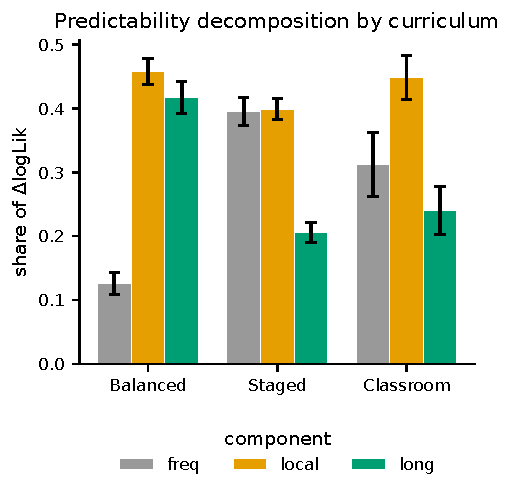
\includegraphics[width=\linewidth]{fig/interp/D5_decomp_shares.pdf}
        \caption{\textbf{Predictability decomposition for balanced vs.\ staged curricula.} Model-level decomposition of the MECO~L2 $\Delta\log L$ into contributions from word log-frequency, local-context surprisal ($k{=}4$ subwords), and long-context surprisal (full passage), averaged across the three MECO languages at each training scale (continual-learning ablations excluded); the three components sum to one. Across all scales, balanced curricula allocate a larger share to long-context information than staged curricula, with the strongest difference at FineWeb-100M ($0.43$ vs.\ $0.09$, $\Delta_\textsc{long}{=}{+}0.34$, $p_\text{perm}{<}10^{-4}$), a smaller but significant difference at 2B ($+0.19$, $p{=}0.010$), and a directionally similar but non-significant difference at 24B ($+0.15$, $p{=}0.080$). The corresponding reduction in staged curricula is largely offset by greater reliance on frequency-based information. Brackets report the long-context share difference together with its label-permutation $p$-value. Results correspond to Tab.~\ref{tab:sig_decomp_curriculum}.}
        \label{fig:D5_decomp_shares}
    \end{subfigure}
    \hfill
    \begin{subfigure}[t]{0.48\linewidth}
        \centering
        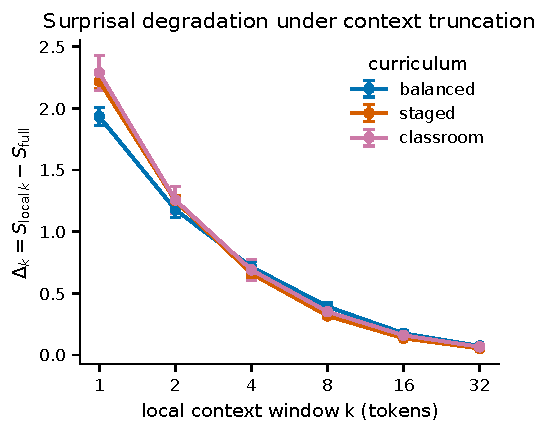
\includegraphics[width=\linewidth]{fig/interp/D6_context_degradation.pdf}
        \caption{\textbf{D6 --- Surprisal degradation under context truncation.} $\Delta_k = S_{\mathrm{local},k} - S_{\mathrm{full}}$ against context window $k$ (B1--B5, nld--eng); larger $\Delta_k$ at small $k$ indicates greater long-range reliance. On average, B1 degrades more than the staged curricula under aggressive truncation.}
        \label{fig:D6_context_degradation}
    \end{subfigure}
    \vspace{0.5em}
    \begin{subfigure}[t]{0.48\linewidth}
        \centering
        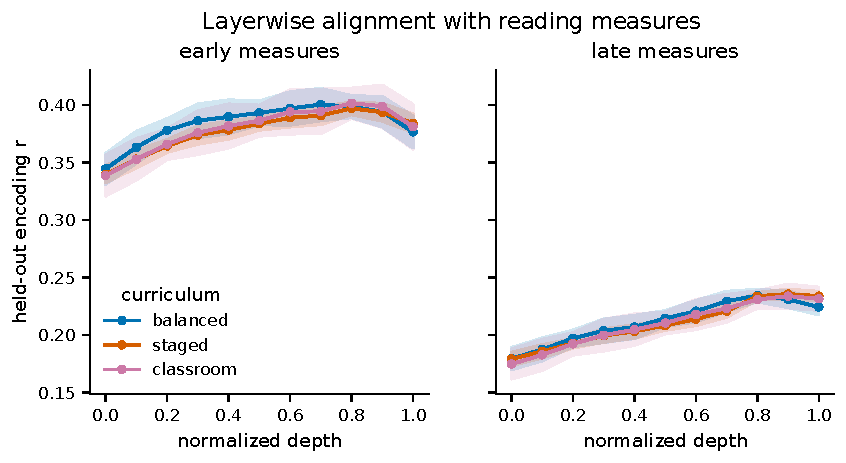
\includegraphics[width=\linewidth]{fig/interp/D8_layerwise_profile.pdf}
        \caption{\textbf{D8 --- Layerwise alignment with reading measures.} Held-out encoding $r$ between layer activations and MECO~L2 measures vs.\ normalized depth ($0$=embedding, $1$=final), one panel per measure; colours = curriculum (B1 vs.\ B3-33, nld--eng FineWeb-100M).}
        \label{fig:D8_layerwise_profile}
    \end{subfigure}
    \hfill
    \begin{subfigure}[t]{0.48\linewidth}
        \centering
        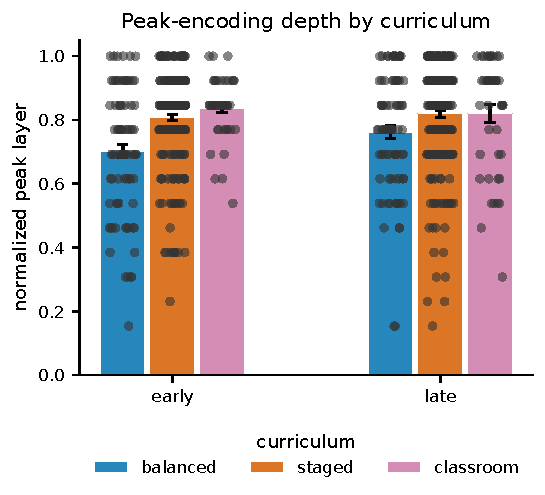
\includegraphics[width=\linewidth]{fig/interp/D9_peak_layer.pdf}
        \caption{\textbf{D9 --- Peak-encoding depth by curriculum.} Normalized depth at which activations align most strongly with each MECO~L2 measure (B1--B5, nld--eng FineWeb-100M). B1 peaks deeper than the staged curricula.}
        \label{fig:D9_peak_layer}
    \end{subfigure}
    \caption{Interpretability analyses across curricula: decomposition of predictability, context dependence, layerwise alignment, and peak encoding depth.}
    \label{fig:interp_grid}
\end{figure*}
 
\begin{figure}[!ht]
    \centering
    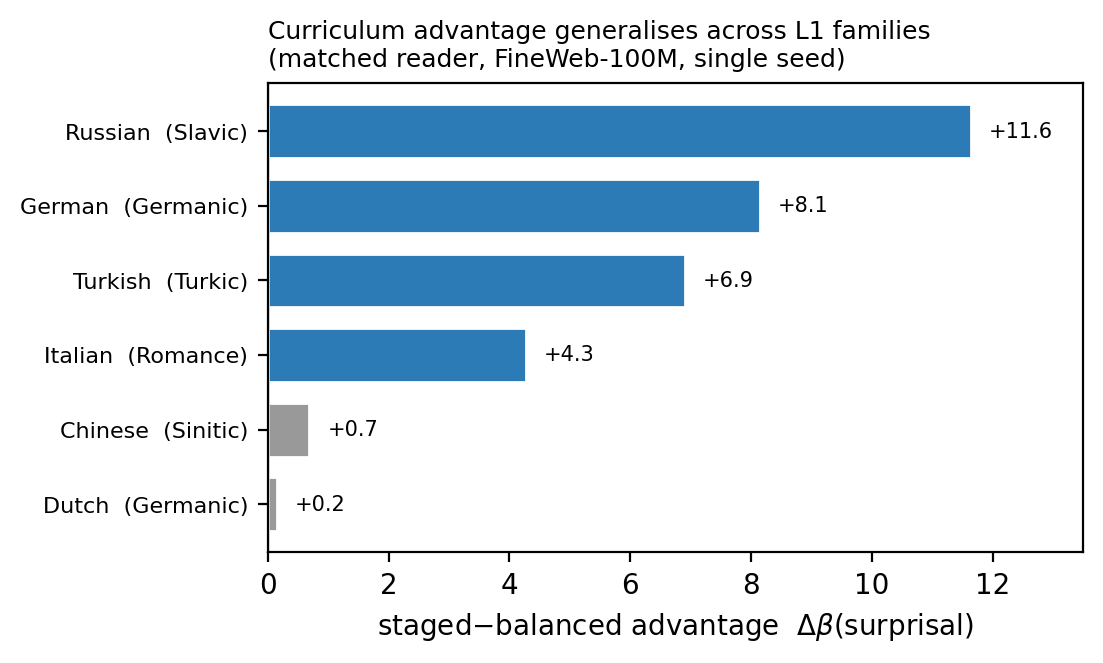
\includegraphics[width=\linewidth]{fig/meco/fig_l1_generality.png}
    \caption{\textbf{Generality of the staged-over-balanced advantage across L1 families.} Per training-L1 advantage $\Delta\beta=\mathrm{mean}(\textrm{B2},\textrm{B3})-\textrm{B1}$ on the cross-cohort-comparable $\beta$(surprisal), each model on its matched reader cohort (FineWeb-100M, single seed). Pooled over six matched L1s, mean $\Delta\beta=+5.3$ (95\% hierarchical-bootstrap CI $[+2.2,+8.5]$, $P{>}0.99$). Single-seed, exploratory.}
    \label{fig:l1_generality}
\end{figure}
 
\paragraph{FLORES training dynamics.} Fig.~\ref{fig:flores_main} tracks FLORES-200 surprisal over training; the catastrophic-forgetting framing is anchored to the per-language table in App.~\ref{sec:downstream} (Tab.~\ref{tab:forgetting}).
 
\begin{figure}[!ht]
    \centering
    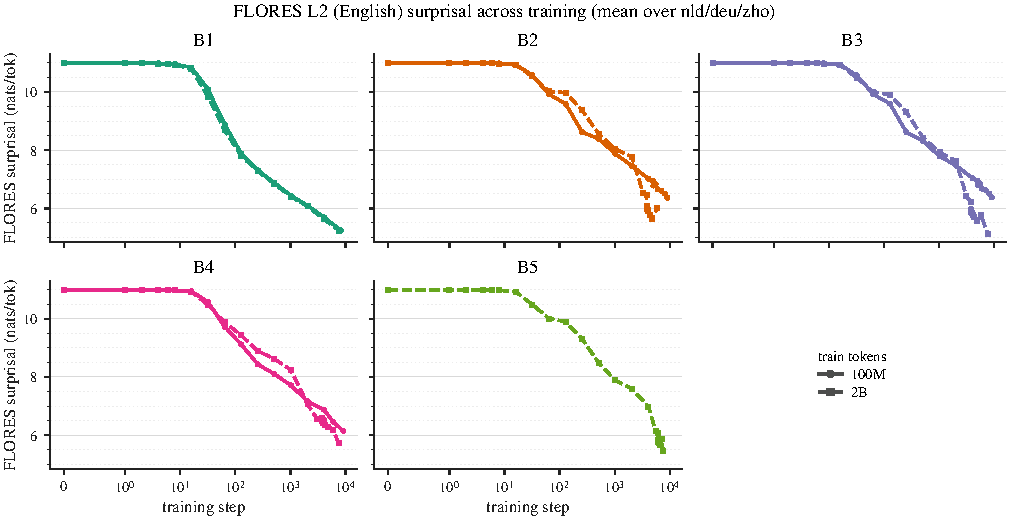
\includegraphics[width=\linewidth]{fig/flores/fig_flores_main.pdf}
    \caption{\textbf{FLORES~L2 (English) surprisal across training.} Mean per-token FLORES-200 surprisal (nats/tok; $\downarrow$ better) against training step (symlog), one panel per curriculum, with 100M (solid) and 2B (dashed) cohorts, averaged over nld/deu/zho. Staged-exposure curricula (B2/B3-33/B5) reach the L2-English surprisal level of the B-GPT reference earlier than B1. L1 retention is summarised separately in Tab.~\ref{tab:forgetting}.}
    \label{fig:flores_main}
\end{figure}
 
\subsection{Cross-model interpretability diagnostics}\label{sec:pico-cross-comp}
 
The Q1 and Q2 analyses constitute the cross-model interpretability diagnostics. Q1 identifies which interpretability metric varies most across L1 and curriculum; Q2 reports how each metric co-varies with the downstream axes over the same cohort. \textbf{All Q2 results are exploratory:} each correlation is over $n=5$ curriculum points on highly correlated curricula, with no significance testing or confidence interval; the $r$-values are hypothesis-generating, not population estimates.
 
\begin{table}[h]
  \centering \small
  \caption{Pearson $r$ across the five nld--eng curricula (B1--B5) for selected (interpretability, downstream) pairs. Bold marks $|r|>0.5$ (descriptive only; with $n{=}5$ this is not a significance threshold). Exploratory.}
  \label{tab:pico-q2-headline}
  \begin{tabular}{lrrrr}
    \toprule
    metric & BLiMP-eng & BLiMP-nl & MECO-du & MECO-ge \\
    \midrule
    $\Vert W_{OV}\Vert_F$       & \textbf{+0.52} & \textbf{$-$0.67} & $-$0.50 & $-$0.49 \\
    Gini$(W_{\text{SwiGLU}})$   & $+$0.36        & \textbf{$-$0.53} & $-$0.31 & $-$0.33 \\
    Hoyer$(W_{\text{SwiGLU}})$  & $+$0.36        & \textbf{$-$0.53} & $-$0.37 & $-$0.33 \\
    $\Vert W_{\text{norm}}\Vert_F$ & $-$0.44     & \textbf{$+$0.60} & \textbf{$+$0.54} & $+$0.42 \\
    $\kappa(W_{OV})$            & $+$0.04        & $-$0.31          & $+$0.06 & $+$0.03 \\
    \bottomrule
  \end{tabular}
\end{table}
 
These metrics are more consistent with a decomposition into partially independent axes than with a single scalar quality dimension. On this sweep, higher Gini/Hoyer/Frobenius on the OV+SwiGLU subspaces co-occurs with higher BLiMP-eng and lower L1 transfer and reading-time alignment. The curriculum with the highest BLiMP-eng (B1) and the one with the highest L1 retention and reading-time alignment (B5) sit at opposite ends of this ($n{=}5$, exploratory) ordering; we leave a fuller investigation to future work.
 
 
% ####################################################################
% ===== BLOCK K --- DOWNSTREAM TASKS =====
% ####################################################################
% =====================================================================
\section{Detailed Downstream Results}\label{sec:downstream}
 
We report \beetle{} \textsc{MultiBLiMP} per-language accuracy (Tab.~\ref{tab:multiblimp}) and catastrophic forgetting by exposure schedule (Tab.~\ref{tab:forgetting}). B3-33 nld--eng reaches the best \beetle{} Dutch grammaticality (90.3\%), and the structured-exposure advantage attenuates across the typological-distance gradient (Dutch~$>$~German~$>$~French~$>$~Persian~$>$~Bulgarian). On FLORES-200, L1 retention after L2 introduction is L1-dependent: B1 balanced retains L1 best on German but is not the least-forgetting schedule on Dutch or Chinese, so no single curriculum minimises the L1 penalty across all three L1s.
 
\begin{table}[!ht]
  \centering \small
  \caption{\textsc{MultiBLiMP} accuracy (\%) across five languages for nld--eng \textsc{HumanScale} \beetle{} models and baselines. Bold = best per column.}
  \label{tab:multiblimp}
  \begin{tabular}{lrrrrr}
    \toprule
    Condition & Dutch & German & French & Persian & Bulg. \\
    \midrule
    \multicolumn{6}{l}{\emph{Monolingual anchors}} \\
    mono-ENG & 53.0 & 60.3 & 60.8 & 52.9 & 63.5 \\
    mono-NLD & 88.9 & 67.4 & 58.9 & 40.4 & 62.4 \\
    \midrule
    \multicolumn{6}{l}{\emph{\beetle{} curricula}} \\
    B1       & 87.6 & 67.6 & 61.5 & 53.4 & 62.5 \\
    B2       & 88.8 & 73.3 & 63.3 & 49.5 & 62.4 \\
    B3-33    & \textbf{90.3} & 72.9 & 62.0 & 51.4 & 62.3 \\
    B3-0     & 89.7 & 70.9 & 61.8 & 51.3 & 62.6 \\
    B4       & 89.8 & 72.3 & 61.5 & 51.6 & 62.3 \\
    B5       & 88.5 & 72.1 & 62.2 & 51.2 & 62.0 \\
    \midrule
    \multicolumn{6}{l}{\emph{BLOOM ladder}} \\
    BLOOM-560m & 59.1 & 65.8 & 81.4 & 55.5 & 58.8 \\
    BLOOM-1b1  & 62.8 & 76.5 & 94.0 & 55.6 & 64.3 \\
    BLOOM-3b   & 65.6 & 80.6 & \textbf{97.9} & 59.9 & 63.9 \\
    BLOOM-7b1  & 64.6 & \textbf{82.7} & 95.3 & \textbf{60.1} & \textbf{67.2} \\
    \bottomrule
  \end{tabular}
\end{table}
 
 
\begin{table}[!ht]
  \centering
  \small
  \setlength{\tabcolsep}{4pt}
  \caption{\textbf{MultiBLiMP Dutch accuracy (\%) by \beetle{} curriculum and training scale, vs.~scale-only baselines on the same target.} \beetle{} (125\,M params) reaches the matched monolingual Dutch anchor at 100\,M tokens (B3-33) and saturates near 96\,\% at 24\,B tokens (B2), surpassing BLOOM-7b1 (7.1\,B params) by $\sim$30\,pp and matching XGLM-4.5B (4.5\,B params) on the same target language. Per-language and per-curriculum breakdowns appear in App.~\ref{sec:downstream}.}
  \label{tab:multiblimp_efficiency}
  \begin{tabular}{l c c c c c}
    \toprule
    & \multicolumn{5}{c}{\beetle{} curriculum (nld--eng)} \\
    \cmidrule(lr){2-6}
    Training scale & B1 & B2 & B3-33 & B4 & B5 \\
    \midrule
    HumanScale 100\,M  & 87.6 & 88.8 & \textbf{90.3} & 89.8 & 88.5 \\
    FineWeb 24\,B      & 94.4 & \textbf{96.0} & ---  & ---  & ---  \\
    \midrule
    \multicolumn{6}{l}{\emph{Baselines (Dutch MultiBLiMP, same eval slice)}} \\
    \multicolumn{5}{l}{\beetle{}-HS mono-Dutch (125\,M, HS 100\,M)} & 88.9 \\
    \multicolumn{5}{l}{BLOOM-7b1 (7.1\,B params, 341\,B tokens)} & 64.6 \\
    \multicolumn{5}{l}{XGLM-4.5B (4.5\,B params, 500\,B tokens)} & 96.9 \\
    \bottomrule
  \end{tabular}
\end{table}
 
 
\paragraph{Catastrophic forgetting.} Tab.~\ref{tab:forgetting} pools (model, L2-language) cells that differ in trajectory length, cell count, and evaluation coverage, so its absolute $\Delta$-PPL and CF log-ratio magnitudes are not comparable across schedules; the five-figure cells reflect \emph{numerical divergence} on a handful of sentences (a run blowing up) rather than graded forgetting, and should be read as ``a run diverged'' rather than ``the model forgot proportionally more.'' Only the within-schedule ordering should be read from this table. L1 retention is best under schedules that keep continuous or rebalanced L1 exposure, and is L1-dependent overall (German retains best; Dutch and Chinese forget on essentially every sentence regardless of curriculum).
 
\begin{table}[!ht]
  \centering \small
  \caption{Catastrophic forgetting aggregated by exposure schedule and L1, sorted by \% sentences worse (ascending). Mean $\Delta$-PPL: mean per-sentence PPL increase over the matched monolingual baseline. CF Log-Ratio: mean log perplexity ratio (positive = worse). $N$ = number of (model, L2-language) cells. Absolute magnitudes are not comparable across schedules; only within-schedule ordering is meaningful.}
  \label{tab:forgetting}
  \begin{tabular}{llrrrr}
    \toprule
    L1 & Schedule & Mean $\Delta$-PPL & CF L-R & \% Worse & $N$ \\
    \midrule
    German  & Balanced     & \textbf{157} & \textbf{+0.14} & \textbf{57} & 2 \\
    German  & Sequential   & 286   & +0.34 & 59  & 2 \\
    German  & Heritage     & 2418  & +0.76 & 67  & 6 \\
    German  & Simultaneous & 1111  & +0.61 & 68  & 4 \\
    German  & Late L2      & 118823 & +3.14 & 93 & 4 \\
    Dutch   & Heritage     & 371   & +2.48 & 100 & 2 \\
    Dutch   & Simultaneous & 774   & +3.17 & 100 & 3 \\
    Dutch   & Balanced     & 1048  & +3.24 & 100 & 8 \\
    Chinese & Late L2      & 1445  & +3.63 & 100 & 5 \\
    Chinese & Balanced     & 7350  & +4.42 & 100 & 9 \\
    Dutch   & Late L2      & 35979 & +4.86 & 100 & 2 \\
    Dutch   & Sequential   & 71758 & +7.66 & 100 & 1 \\
    \bottomrule
  \end{tabular}
\end{table}
 
 
% =====================================================================
\section{Supplementary BLiSS and Pedagogical Results}\label{sec:supp-results}
 
\subsection{BLiSS supplementary results}\label{appcomp:bliss}
 
The BLiSS view of the curriculum trade-off is the final-checkpoint relationship between BLiSS RP$@0$ and MECO~L2 $\Delta\log L$: the curriculum ordering on BLiSS runs opposite to the MECO~L2 ordering. We read the trade-off from the \emph{within-\beetle{}} scatter (Fig.~\ref{fig:bliss_vs_meco_beetle}), which drops the LLM baselines and monolingual anchors so that only models sharing one tokeniser and aggregation are compared: across the $n{=}33$ matched cells the relationship is negative and significant (Spearman $\rho={-}0.47$, $p{=}6.3{\times}10^{-3}$; Pearson $r={-}0.37$), consistent with the matched-curriculum ordering B3-33~$>$~B5~$>$~B2~$>$~B4~$>$~B1 on FineWeb nld--eng RP$@0$.
 
\begin{figure}[!ht]
  \centering
  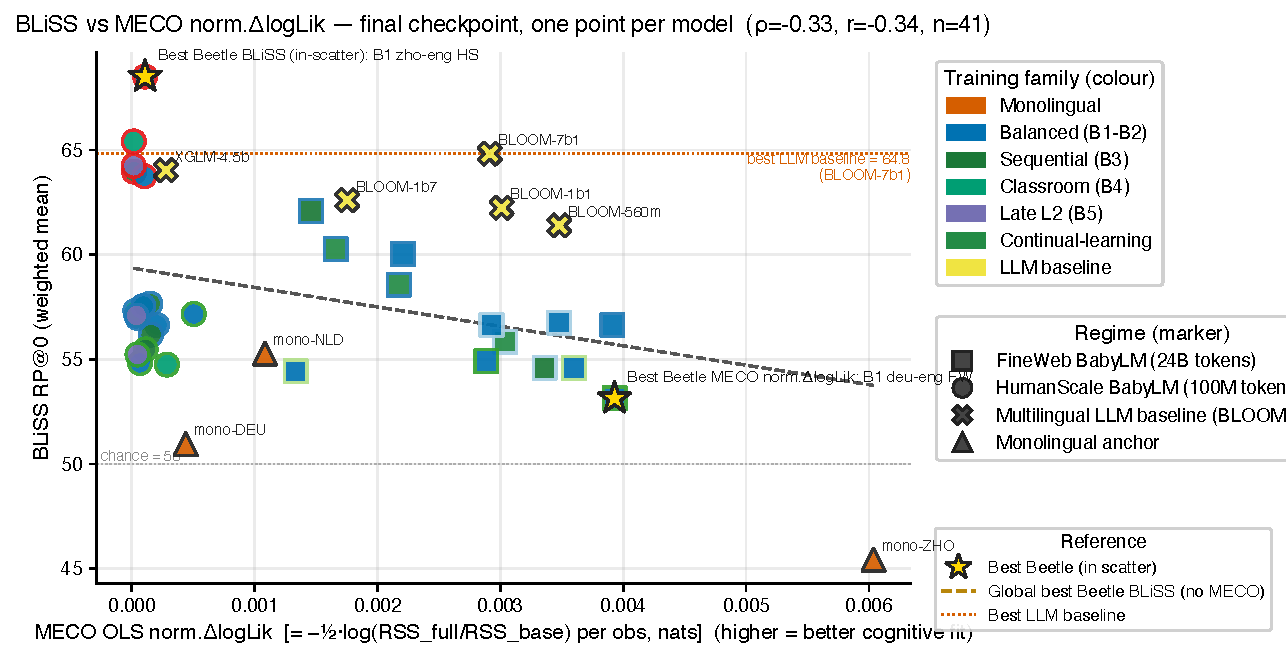
\includegraphics[width=\linewidth]{fig/fig_bliss_vs_meco_final.pdf}
  \caption{\textbf{Within-\beetle{} BLiSS RP$@0$ vs.\ MECO~L2 $\Delta\log L$ (final checkpoint, matched models only).} Each point is one \beetle{} curriculum$\times$L1$\times$scale cell; LLM baselines and monolingual anchors are excluded, so the trade-off rests on models sharing one tokeniser and aggregation (Spearman $\rho={-}0.47$, $p{=}6.3{\times}10^{-3}$, $n{=}33$). This is the form we recommend reading the trade-off from.}
  \label{fig:bliss_vs_meco_beetle}
\end{figure}
 
\subsection{Pedagogical supplementary results}\label{appcomp:peda}
 
Tab.~\ref{tab:headline_pedagogical} summarises the downstream performance of \beetle{} 125M models on CLOTH closed-cloze accuracy, Cambridge open-cloze accuracy, JFLEG learner-fluency margin, false-friend disambiguation margin, and the CEFR perplexity gradient, by curriculum and training scale.
 
\begin{table*}[!ht]
  \centering \scriptsize
  \setlength{\tabcolsep}{4pt}
  \caption{\textbf{Downstream pedagogical performance of \beetle{} models.} CLOTH closed-cloze accuracy, Cambridge open-cloze accuracy, JFLEG learner-fluency margin (bits/token; positive = model prefers corrected over learner-error sentence), false-friend disambiguation margin (bits/token), CEFR-A1 / CEFR-C2 BPT, and CEFR gradient. Bold = best per column within the matched-L1 nld--eng family.}
  \label{tab:headline_pedagogical}
  \begin{tabular}{llrrrrrrr}
    \toprule
    Model & Family & CLOTH & Camb.~OC & JFLEG & FF & A1 BPT & C2 BPT & A1$\to$C2 \\
    \midrule
    B1 nld--eng     & HS & \textbf{0.380} & \textbf{0.644} & \textbf{0.949} & \textbf{0.585} & 6.572 & 8.818 & 2.247 \\
    B2 nld--eng     & HS & 0.302 & 0.596 & 0.750 & 0.156 & 8.051 & 10.213 & 2.163 \\
    B3-33 nld--eng  & HS & 0.310 & 0.587 & 0.751 & 0.174 & 8.106 & 10.275 & 2.169 \\
    B4 nld--eng     & HS & 0.304 & 0.582 & 0.801 & $-$0.055 & 7.719 & 9.755 & 2.036 \\
    B5 nld--eng     & HS & 0.302 & 0.584 & 0.716 & 0.238 & 8.127 & 10.193 & 2.066 \\
    \midrule
    B1 nld--eng     & FW-2B & 0.369 & 0.638 & 0.833 & 0.457 & 8.851 & 8.614 & $-$0.237 \\
    B2 nld--eng     & FW-2B & 0.322 & 0.567 & 0.502 & 0.238 & 10.317 & 11.047 & 0.730 \\
    B3-33 nld--eng  & FW-2B & 0.329 & 0.614 & 0.511 & 0.235 & 10.354 & 11.056 & 0.702 \\
    B5 nld--eng     & FW-2B & 0.323 & 0.570 & 0.509 & 0.318 & 10.364 & 11.040 & 0.676 \\
    \midrule
    mono-eng        & HS & 0.369 & 0.659 & 0.888 & 0.351 & 7.297 & 10.558 & \textbf{3.261} \\
    mono-nld        & HS & 0.267 & 0.310 & 0.306 & $-$0.034 & 9.875 & 10.671 & 0.796 \\
    \bottomrule
  \end{tabular}
\end{table*}
 
 
% ####################################################################
% ===== BLOCK L --- CROSS-LINGUAL / PRIMING =====
% ####################################################################
% =====================================================================
\section{Cross-lingual Structural Priming (B-GPT Comparison)}\label{sec:priming}
 
As a convergent check that \beetle{} reproduces known bilingual behaviour, we evaluate \emph{cross-lingual structural priming} on the Dutch--English benchmark of \citet{bernolet2013language} (genitive alternations; $96$ items per condition). A between-language priming effect (prime in one language, target in the other) requires \emph{shared}, not merely parallel, structural representations across the two training languages. We quantify priming with the normalised relative probability the model assigns the target under the matching prime,
\[
  P_N(i) = \frac{\exp\!\big({-}\mathrm{Surp}_{\text{match}}(t_i)\big)}
                {\exp\!\big({-}\mathrm{Surp}_{\text{match}}(t_i)\big) + \exp\!\big({-}\mathrm{Surp}_{\text{mismatch}}(t_i)\big)},
\]
so $P_N=0.5$ is no priming and $P_N>0.5$ a facilitatory effect. Significance is from a paired $t$-test of $P_N-0.5$ against zero (corroborated by a $10{,}000$-sample sign-flip permutation); inference is at the \emph{item} level. Curricula are single-seed, so we do not claim curriculum priming differences generalise across re-trainings. This is a validation diagnostic, not a principal claim.
 
\paragraph{Within-\beetle{} priming is robust.} Table~\ref{tab:priming_within_model} reports final-checkpoint within-model $P_N$ for the FineWeb nld--eng curricula. Every curriculum shows above-chance facilitation in \emph{both} directions, significant in $9$ of the $10$ cells; the sole exception is B3-33 Dutch$\to$English ($P_N=0.56$, $p=0.05$), which is borderline. The English$\to$Dutch direction is in fact the more significant for B2, B4, and B5, so $P_N$ shows no systematic Dutch$\to$English advantage on these cells.
 
\begin{table}[!ht]
  \centering \small
  \caption{\textbf{Within-\beetle{} cross-lingual priming (Bernolet, FineWeb nld--eng, final checkpoint).} Mean $P_N$ ($0.5=$ no priming), paired $t$ of $P_N-0.5$ vs.\ zero, and its $p$ ($n{=}192$ items per cell).}
  \label{tab:priming_within_model}
  \begin{tabular}{llrrr}
    \toprule
    Curriculum & Direction & mean $P_N$ & $t$ & $p$ \\
    \midrule
    B1    & D$\to$E & $0.599$ & $3.62$ & $3.8{\times}10^{-4}$ \\
    B1    & E$\to$D & $0.594$ & $3.91$ & $1.3{\times}10^{-4}$ \\
    B2    & D$\to$E & $0.562$ & $2.10$ & $0.037$ \\
    B2    & E$\to$D & $0.629$ & $7.80$ & $<10^{-4}$ \\
    B3-33 & D$\to$E & $0.559$ & $1.97$ & $0.051$ \\
    B3-33 & E$\to$D & $0.581$ & $4.55$ & $1.0{\times}10^{-5}$ \\
    B4    & D$\to$E & $0.597$ & $3.44$ & $7.2{\times}10^{-4}$ \\
    B4    & E$\to$D & $0.639$ & $6.76$ & $<10^{-4}$ \\
    B5    & D$\to$E & $0.603$ & $3.77$ & $2.2{\times}10^{-4}$ \\
    B5    & E$\to$D & $0.600$ & $5.56$ & $<10^{-4}$ \\
    \bottomrule
  \end{tabular}
\end{table}
 
\paragraph{\beetle{} reproduces B-GPT-level priming under broader curriculum coverage.} Fig.~\ref{fig:priming_finalckpt} sets final-checkpoint Bernolet priming for \beetle{} against the B-GPT schedules of \citet{arnett-etal-2025-acquisition}. \beetle{}'s best curricula are competitive with B-GPT's strongest schedules, which B-GPT-sequential edges by a small margin at the final checkpoint. The point is not that \beetle{} wins: B-GPT samples two curricula whereas \beetle{} realises comparable priming across four schedules (B1--B3, B5), so the effect is not an artefact of a single schedule. The B-GPT comparison is \emph{descriptive only}: the public B-GPT release provides aggregate per-language-pair means, not per-item surprisals, so paired item-level inference against B-GPT is not possible.
 
\begin{figure}[!ht]
  \centering
  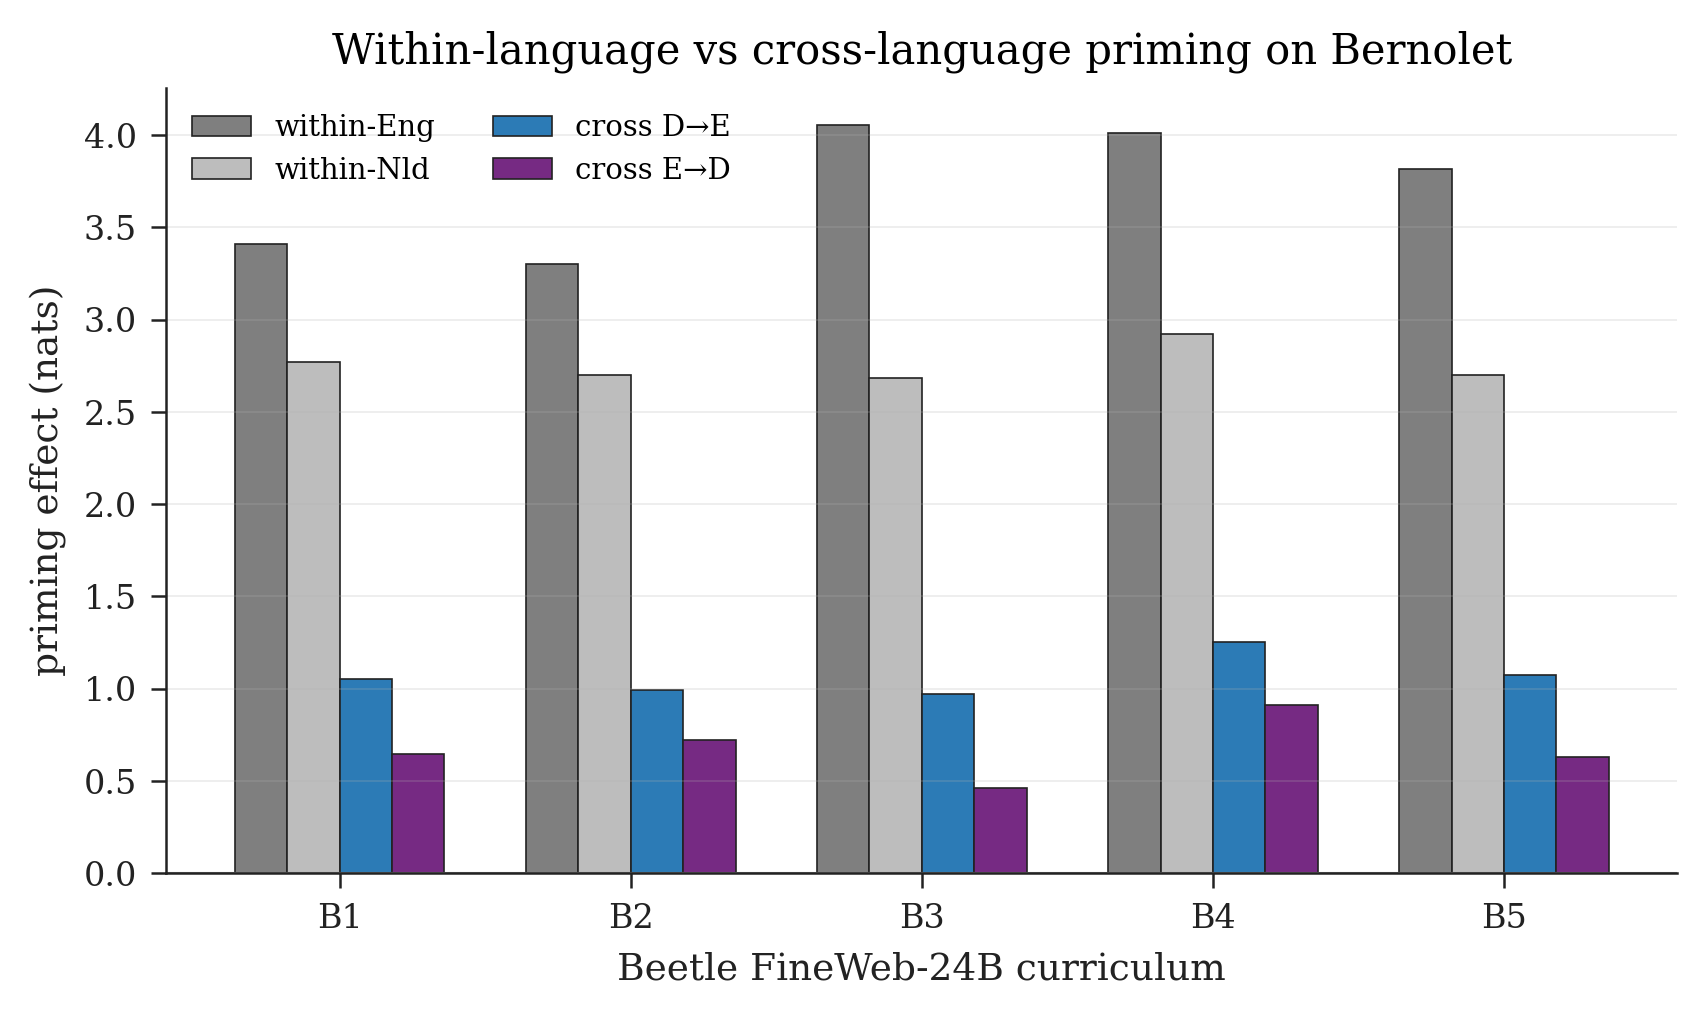
\includegraphics[width=\linewidth]{fig/priming/fig_within_vs_cross_bernolet.png}
  \caption{\textbf{Final-checkpoint cross-lingual priming (Bernolet).} Between-language priming for \beetle{} FineWeb curricula (B1--B3, B5) and the B-GPT simultaneous/sequential schedules. \beetle{} is competitive across four curricula; B-GPT-sequential slightly exceeds the best \beetle{} condition. Descriptive cross-class comparison (no per-item B-GPT inference).}
  \label{fig:priming_finalckpt}
\end{figure}
 
\begin{figure}[!ht]
  \centering
  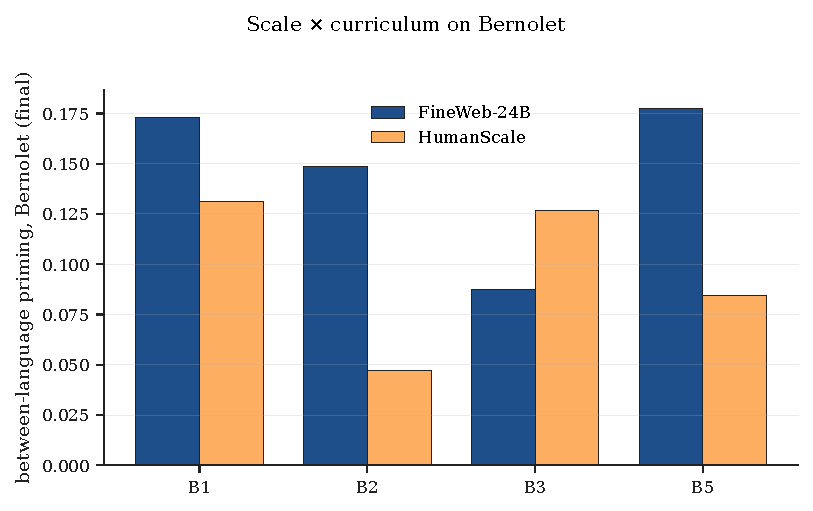
\includegraphics[width=\linewidth]{fig/priming/fig_main_humanscale_bernolet.pdf}
  \caption{\textbf{Priming trajectory (Bernolet), training-time normalised.} Between-language priming vs.\ fraction of training for \beetle{} curricula (B1--B3, B5) and B-GPT. Both families transition into a non-trivial effect --- B-GPT-sequential step-jumps at its L1$\to$L2 boundary, \beetle{} rises more smoothly --- and converge by end of training.}
  \label{fig:priming_trajectory}
\end{figure}
